% Options for packages loaded elsewhere
\PassOptionsToPackage{unicode}{hyperref}
\PassOptionsToPackage{hyphens}{url}
\PassOptionsToPackage{dvipsnames,svgnames,x11names}{xcolor}
%
\documentclass[
]{article}
\usepackage{amsmath,amssymb}
\usepackage{iftex}
\ifPDFTeX
  \usepackage[T1]{fontenc}
  \usepackage[utf8]{inputenc}
  \usepackage{textcomp} % provide euro and other symbols
\else % if luatex or xetex
  \usepackage{unicode-math} % this also loads fontspec
  \defaultfontfeatures{Scale=MatchLowercase}
  \defaultfontfeatures[\rmfamily]{Ligatures=TeX,Scale=1}
\fi
\usepackage{lmodern}
\ifPDFTeX\else
  % xetex/luatex font selection
\fi
% Use upquote if available, for straight quotes in verbatim environments
\IfFileExists{upquote.sty}{\usepackage{upquote}}{}
\IfFileExists{microtype.sty}{% use microtype if available
  \usepackage[]{microtype}
  \UseMicrotypeSet[protrusion]{basicmath} % disable protrusion for tt fonts
}{}
\makeatletter
\@ifundefined{KOMAClassName}{% if non-KOMA class
  \IfFileExists{parskip.sty}{%
    \usepackage{parskip}
  }{% else
    \setlength{\parindent}{0pt}
    \setlength{\parskip}{6pt plus 2pt minus 1pt}}
}{% if KOMA class
  \KOMAoptions{parskip=half}}
\makeatother
\usepackage{xcolor}
\usepackage{longtable,booktabs,array}
\usepackage{calc} % for calculating minipage widths
% Correct order of tables after \paragraph or \subparagraph
\usepackage{etoolbox}
\makeatletter
\patchcmd\longtable{\par}{\if@noskipsec\mbox{}\fi\par}{}{}
\makeatother
% Allow footnotes in longtable head/foot
\IfFileExists{footnotehyper.sty}{\usepackage{footnotehyper}}{\usepackage{footnote}}
\makesavenoteenv{longtable}
\usepackage{graphicx}
\makeatletter
\newsavebox\pandoc@box
\newcommand*\pandocbounded[1]{% scales image to fit in text height/width
  \sbox\pandoc@box{#1}%
  \Gscale@div\@tempa{\textheight}{\dimexpr\ht\pandoc@box+\dp\pandoc@box\relax}%
  \Gscale@div\@tempb{\linewidth}{\wd\pandoc@box}%
  \ifdim\@tempb\p@<\@tempa\p@\let\@tempa\@tempb\fi% select the smaller of both
  \ifdim\@tempa\p@<\p@\scalebox{\@tempa}{\usebox\pandoc@box}%
  \else\usebox{\pandoc@box}%
  \fi%
}
% Set default figure placement to htbp
\def\fps@figure{htbp}
\makeatother
\setlength{\emergencystretch}{3em} % prevent overfull lines
\providecommand{\tightlist}{%
  \setlength{\itemsep}{0pt}\setlength{\parskip}{0pt}}
\setcounter{secnumdepth}{5}
\usepackage{booktabs}

\usepackage[a4paper, margin=2cm]{geometry}

\usepackage{fontawesome5}
\usepackage{xcolor}
\usepackage{framed}
\usepackage{tcolorbox}

% Define colors
\definecolor{infocolor}{RGB}{209, 236, 241}
\definecolor{infoborder}{RGB}{190, 229, 235}
\definecolor{warningcolor}{RGB}{255, 243, 205}
\definecolor{warningborder}{RGB}{255, 234, 167}
\definecolor{tipcolor}{RGB}{212, 237, 218}
\definecolor{tipborder}{RGB}{195, 230, 203}
\definecolor{errorcolor}{RGB}{248, 215, 218}
\definecolor{errorborder}{RGB}{245, 198, 203}

% Define box environments
\newtcolorbox{infobox}{
  colback=infocolor,
  colframe=infoborder,
  boxrule=1pt,
  arc=3pt,
  left=10pt,
  right=10pt,
  top=10pt,
  bottom=10pt
}

\newtcolorbox{warningbox}{
  colback=warningcolor,
  colframe=warningborder,
  boxrule=1pt,
  arc=3pt,
  left=10pt,
  right=10pt,
  top=10pt,
  bottom=10pt
}

\newtcolorbox{tipbox}{
  colback=tipcolor,
  colframe=tipborder,
  boxrule=1pt,
  arc=3pt,
  left=10pt,
  right=10pt,
  top=10pt,
  bottom=10pt
}

\newtcolorbox{errorbox}{
  colback=errorcolor,
  colframe=errorborder,
  boxrule=1pt,
  arc=3pt,
  left=10pt,
  right=10pt,
  top=10pt,
  bottom=10pt
}

% Bibliography formatting
\usepackage{titlesec}
\titleformat{\chapter}[display]
  {\normalfont\huge\bfseries}{\chaptertitlename\ \thechapter}{20pt}{\Huge}
\titlespacing*{\chapter}{0pt}{-50pt}{40pt}

% Control page breaks before bibliography
\let\oldbibliography\bibliography
\renewcommand{\bibliography}[1]{%
  \clearpage
  \phantomsection
  \oldbibliography{#1}
}
\usepackage{fontawesome5}
\usepackage[]{natbib}
\bibliographystyle{apalike}
\nocite{*}
\usepackage{bookmark}
\IfFileExists{xurl.sty}{\usepackage{xurl}}{} % add URL line breaks if available
\urlstyle{same}
\hypersetup{
  pdftitle={IRR Calculator Tutorial},
  pdfauthor={Joe Hightower},
  colorlinks=true,
  linkcolor={blue},
  filecolor={Maroon},
  citecolor={Blue},
  urlcolor={blue},
  pdfcreator={LaTeX via pandoc}}

\title{IRR Calculator Tutorial}
\author{Joe Hightower}
\date{2025-06-12}

\begin{document}
\maketitle

{
\hypersetup{linkcolor=}
\setcounter{tocdepth}{2}
\tableofcontents
}
\section{Introduction}\label{introduction}

This is a short book intended to function as tutorial for the IAQG App ``IRR Calculator''. We will, however, present some of the detail and theory behind the IRR and discuss applications of the Calculator. Our goal is to help both Design Engineers and Quality Engineers apply the IRR Calculator to identify appropriate IRR values and to guide future designs to manage the effects of design decisions on manufacturing efforts

\subsection{IRR Calculator App}\label{irr-calculator-app}

This Tutorial provides both an understanding of the features and capabilities of the Tool. This will help the user gain the most from using the tool.

But the most important aspect of the tool is the questions that the tool can help the Design Engineer and Quality Engineer can answer. Each can benefit from the ability of the tool to relate real decision problems in Design and Quality

\subsubsection{Using The Tool}\label{using-the-tool}

To help a user understand how the app works including how the calculator works and how contour plots work. This purpose is primarily about function. These include questions like:

\begin{enumerate}
\def\labelenumi{\arabic{enumi}.}
\tightlist
\item
  What inputs are required?
\item
  What boundary conditions are enforced by the tool
\item
  How to use the different tabs for the calculator and the design space analysis
\item
  How to use the graphical toolbar included with the contour plots in the design space analysis?
\end{enumerate}

\subsubsection{The Design Engineering Tasks}\label{the-design-engineering-tasks}

The Design Engineer will ask how the IRR relates to design decisions that affect the two parameters Probability of Failure given Conformance and the Probability of Failure Given Nonconformance. More importantly, how do these choices affect the inspection system requirements that must be applied to the manufacturing system.

The Design Engineer has two primary tasks for which this tool will prove beneficial:

\begin{enumerate}
\def\labelenumi{\arabic{enumi}.}
\tightlist
\item
  The design process - making design decisions that affect the Probability of Failure when conforming (closely related to margins of safety) and decisions that affect the Probability of Failure when nonconforming (closely related to fault tolerant design)
\item
  Evaluating possible IRR values for and existing product - many existing products were not designed with the IRR in mind. But the design engineer may be asked to assign an IRR. This process will require at a minimum a qualitative, heuristics driven process to assess original goal for the maximum allowable probability of failure required by the delivered product. they will also need to assign estimates to the probability of failure given conformance and probability of failure given nonconformance and then the IRR that results from these three inputs. Of course a process like this has risk for cognitive bias and is subject to significant epistemic uncertainty
\end{enumerate}

\subsubsection{The Quality Engineering Tasks}\label{the-quality-engineering-tasks}

The Quality Engineering Task is two fold. First, the quality Engineer designs the Inspection System which in conjunction with the manufacturing processes will manage the realized probability of conformance in delivered product (the outgoing quality).

Second, the Quality Engineer may be required to evaluate a proposed IRR (such as those provided in Appendix A of AS9138) for a given application. To make that assessment, the Quality Engineer will be helped by understanding the three relevant questions the Quality Engineer must be prepared to answer:

\begin{enumerate}
\def\labelenumi{\arabic{enumi}.}
\tightlist
\item
  What order of magnitude is associated with the target maximum probability of failure that the Design Engineer associates with the selected characteristic.
\item
  what is the relationship between the probability of failure given conformance for the existing design and the proposed IRR values selected?
\item
  what is the relationship between the probability of failure given nonconformance for the existing design and the proposed IRR values selected?
\item
  what is the relationship between the probability of failure given conformance and the probability of failure given nonconformance
\end{enumerate}

\subsection{Chapter summaries}\label{chapter-summaries}

\begin{enumerate}
\def\labelenumi{\arabic{enumi}.}
\tightlist
\item
  Chapter 1 Presents a general overview of the purpose of this app
\item
  Chapter 2 Discusses the relationship between reliability results and manufacturing outputs
\item
  Chapter 3 Presents the IRR equation, the mathematical development, and the enforceable boundary conditions
\item
  Chapter 4 Discusses the IRR Calculator and offers several examples of applications
\item
  Chapter 5 Discusses the Design Space Analysis Tools and offers several examples of Applications
\item
  Chapter 6 Presents additional useful notes
\item
  Chapter 7 Provides a glossary for terms that may be less familiar to the users
\item
  Chapter 8 adds a list of relevant references used in the development of the Tutorial
\end{enumerate}

\subsection{Notes on the bookdown Interface}\label{notes-on-the-bookdown-interface}

This Tutorial is presented using the bookdown interface \citep{R-bookdown}. There are several features of the bookdown interface used to display the book that are useful to understand. We present an overview here:

The main interface is shown in the next Figure. There a few simple controls that may prove useful to the user.

\begin{figure}

{\centering 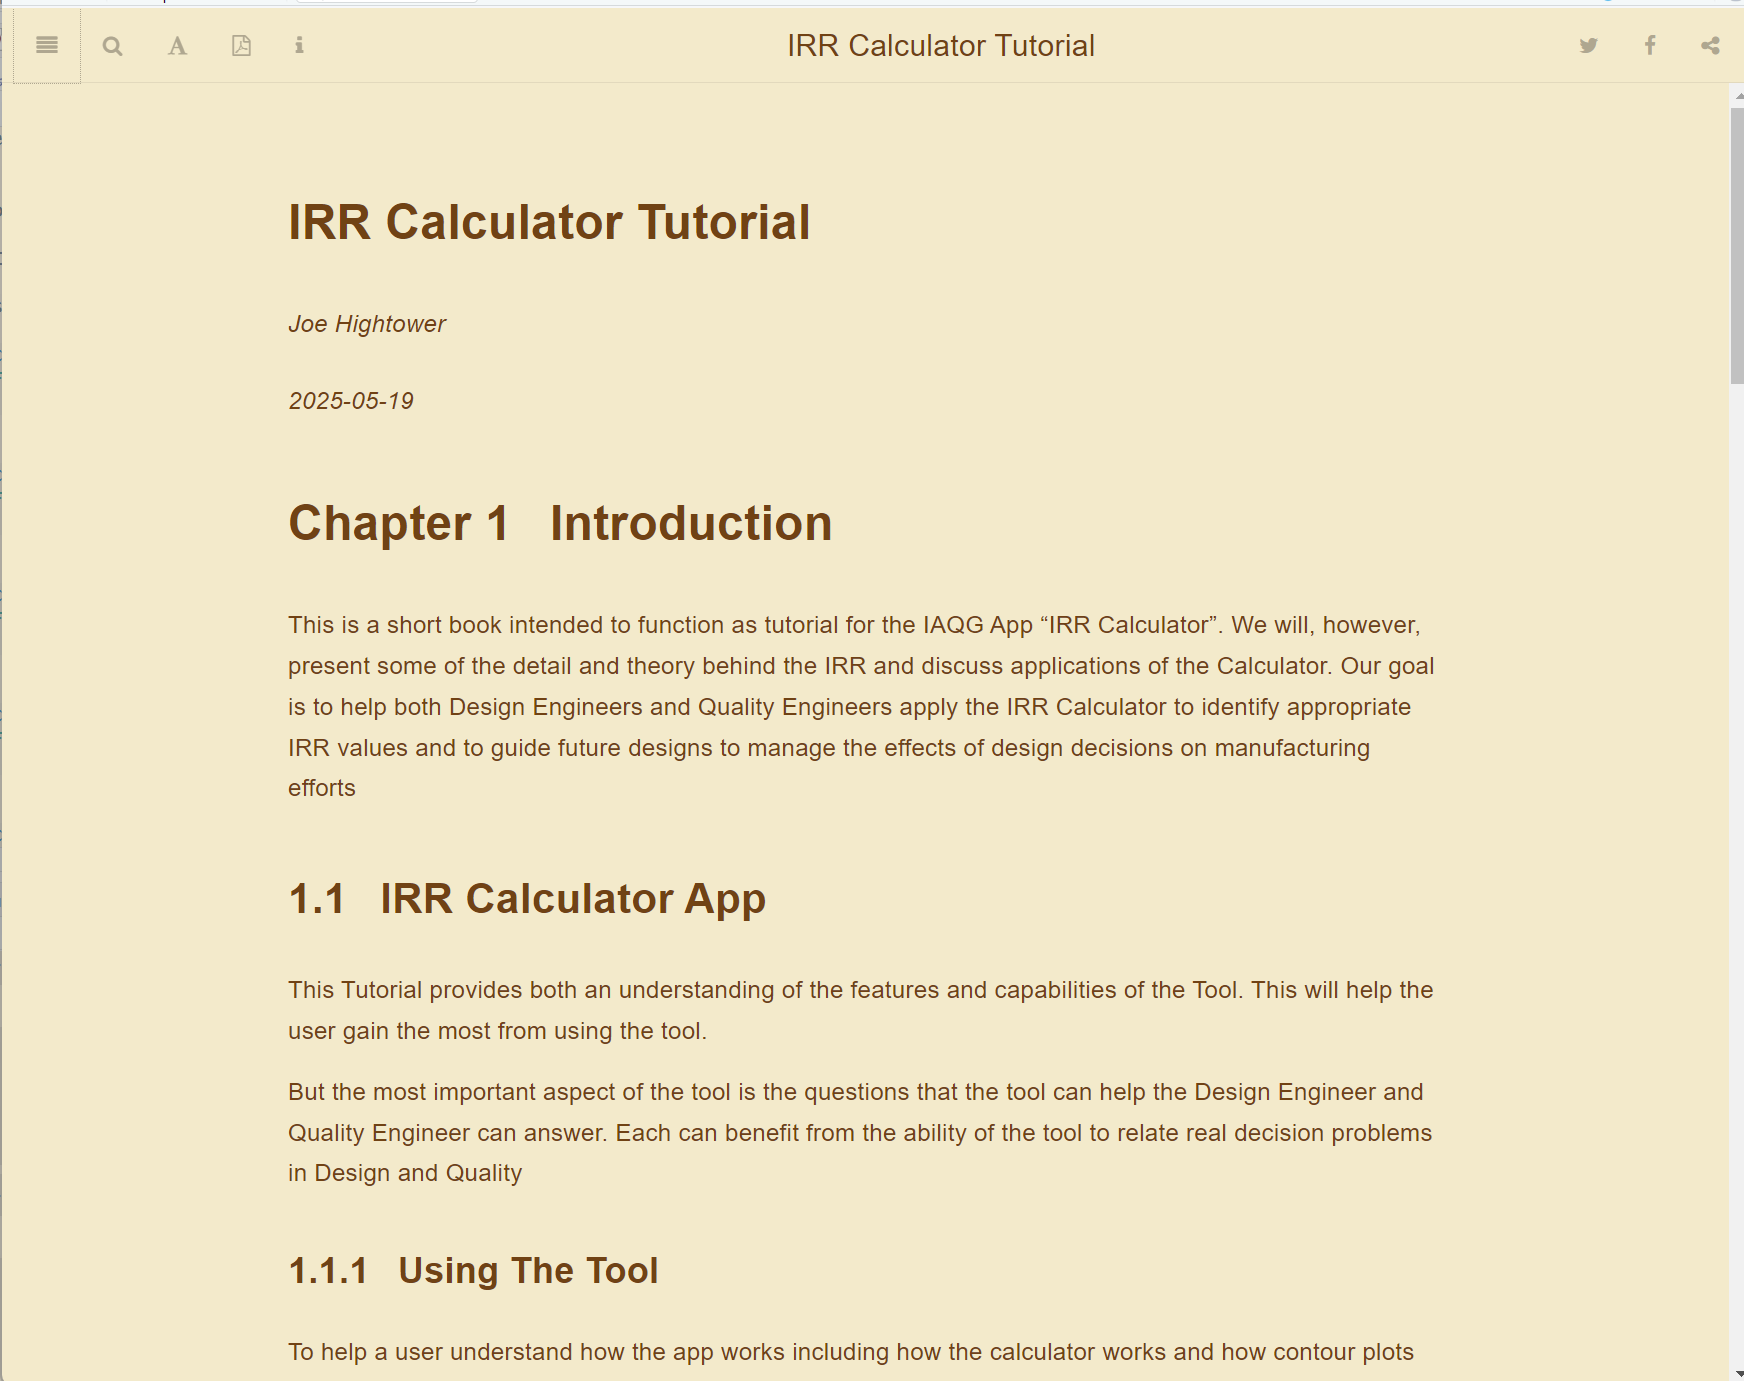
\includegraphics[width=0.5\linewidth]{Main Book Interface} 

}

\caption{Main bookdown Interface}\label{fig:unnamed-chunk-2}
\end{figure}

The Table of Contents can be made visible or hidden depending on preference:

\begin{figure}

{\centering 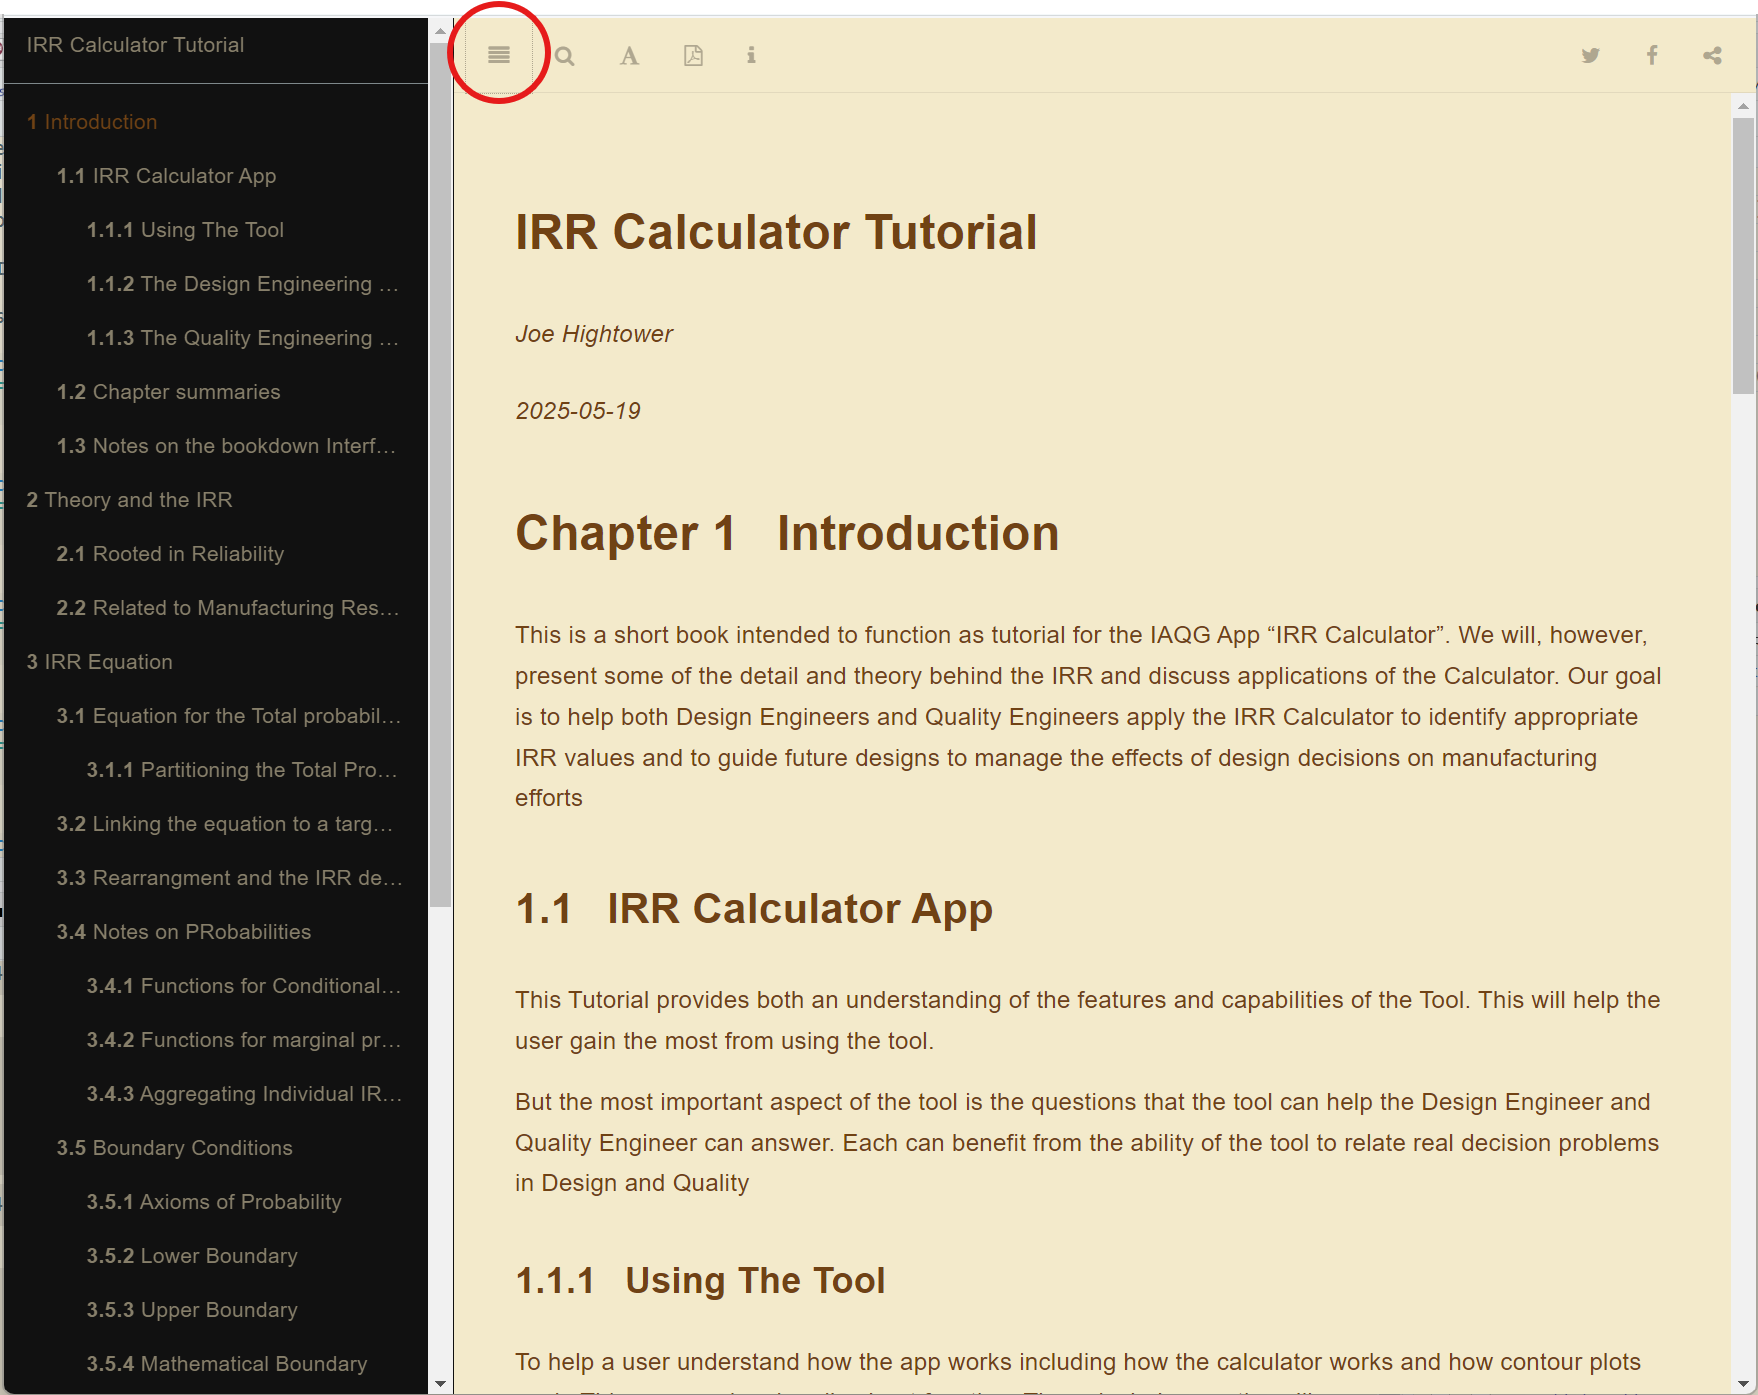
\includegraphics[width=0.5\linewidth]{Table of Contents Sidebar} 

}

\caption{The Table of Contents Sidebar}\label{fig:unnamed-chunk-3}
\end{figure}

The book can be searched using this icon. Text is entered at the top of the Table of Contents Bar:

\begin{figure}

{\centering 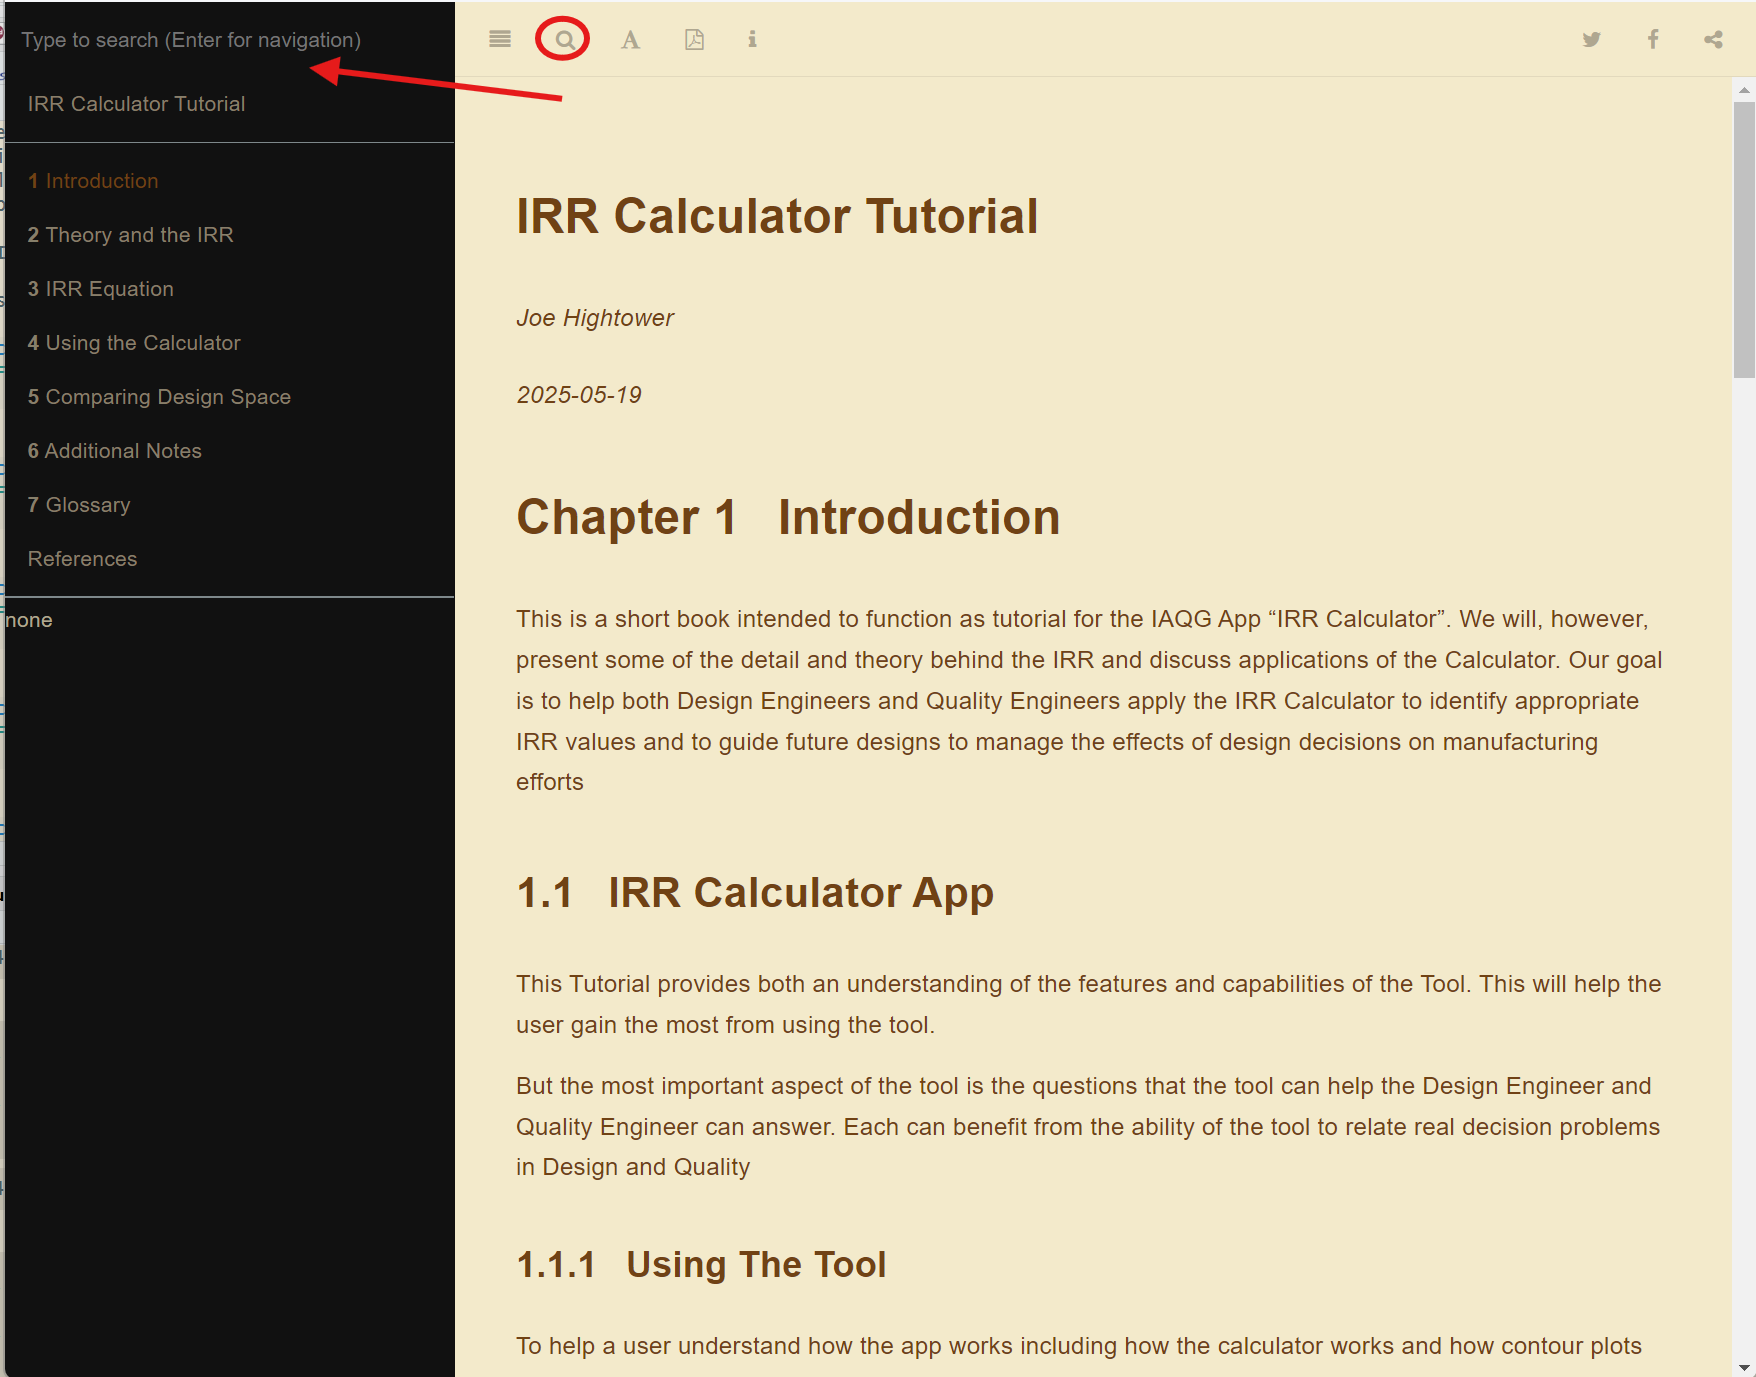
\includegraphics[width=0.5\linewidth]{Search Bar} 

}

\caption{Search Bar}\label{fig:unnamed-chunk-4}
\end{figure}

The App provides a few tools to manage font size, background color, line spacing, and font type:

\begin{figure}

{\centering 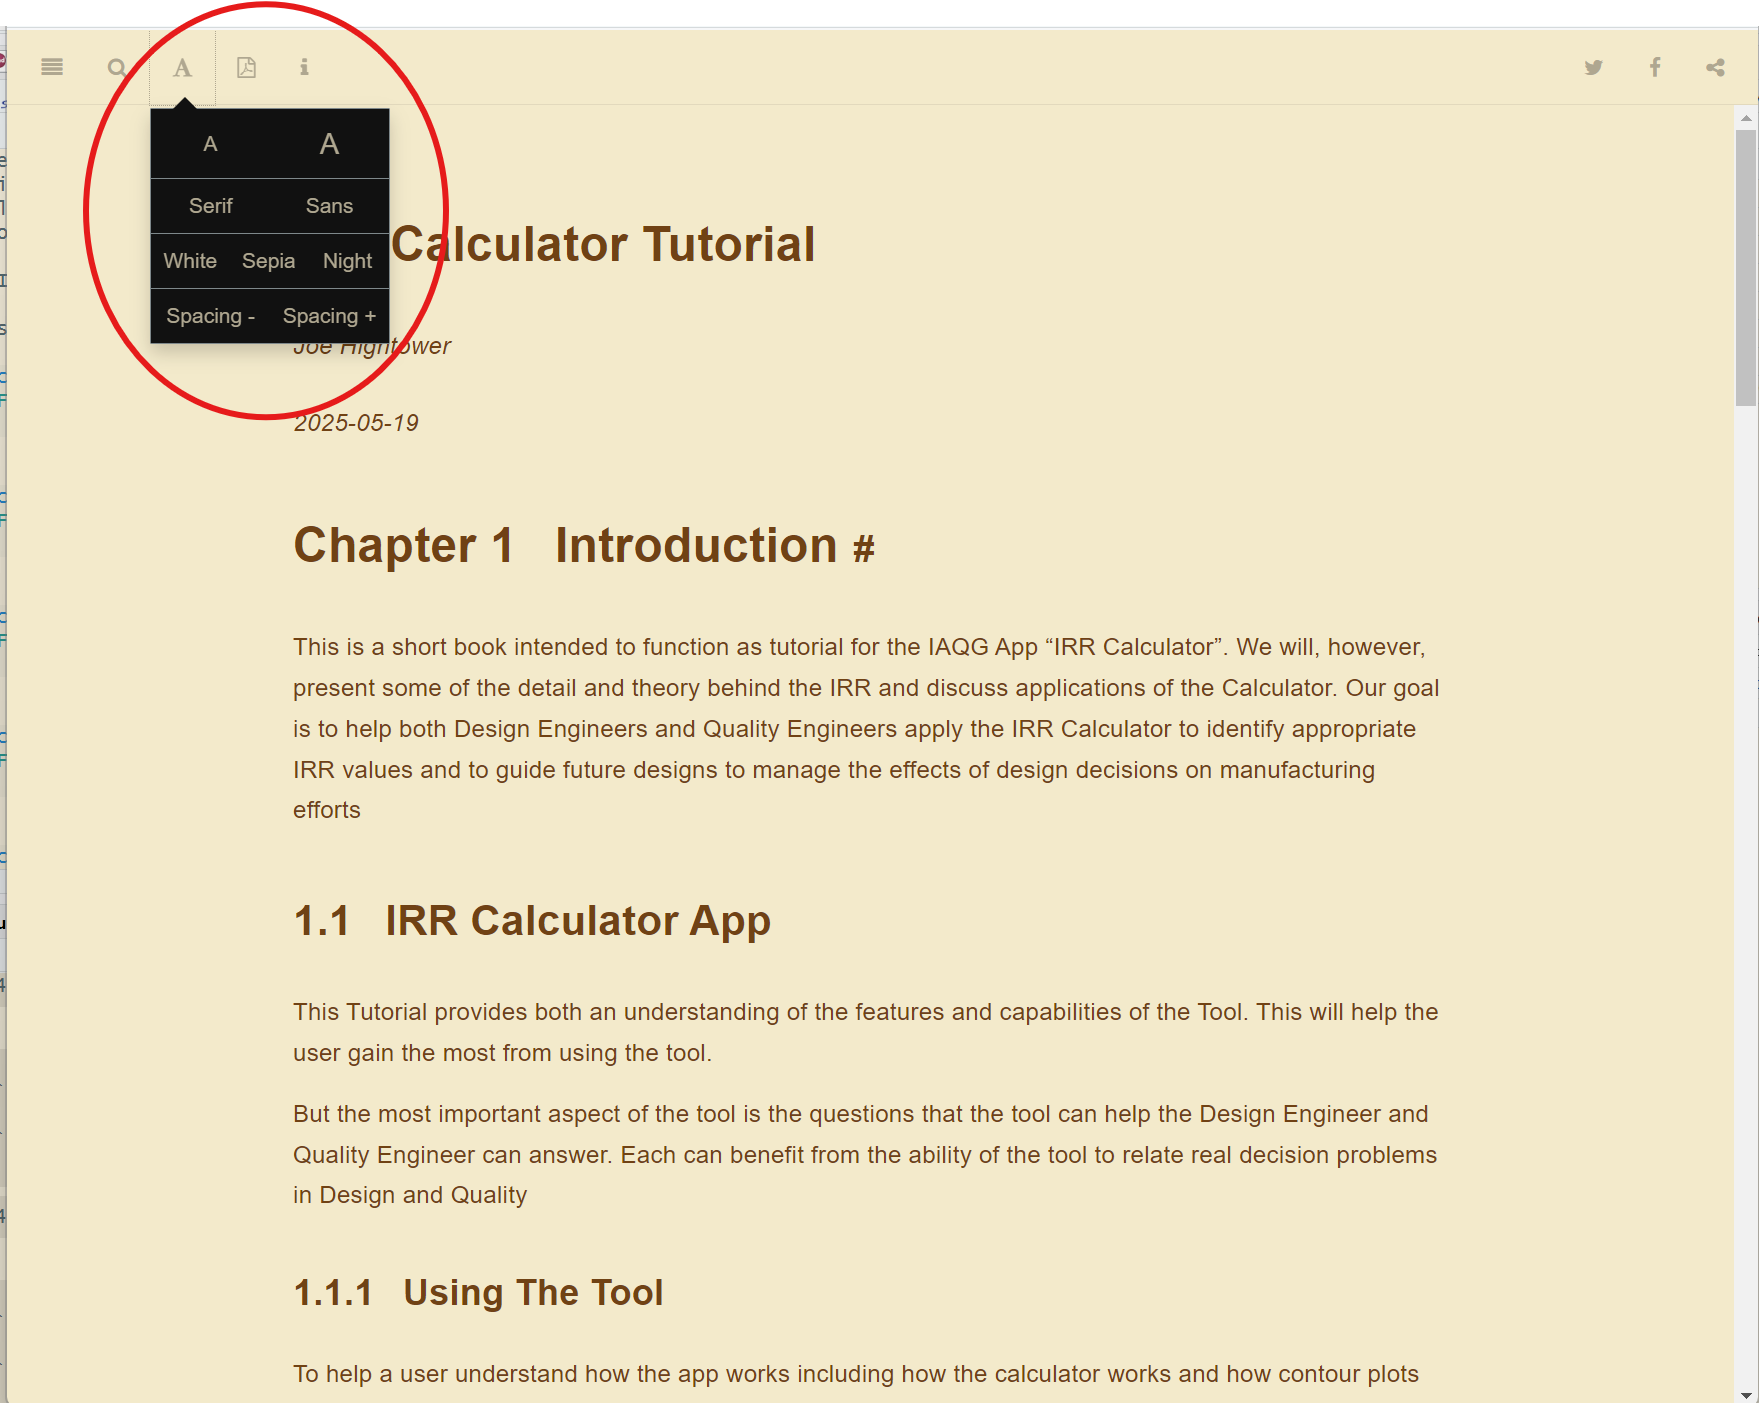
\includegraphics[width=0.5\linewidth]{Font Management} 

}

\caption{Font Management}\label{fig:unnamed-chunk-5}
\end{figure}

This selection will allow the user to download a pdf copy of this book:

\begin{figure}

{\centering 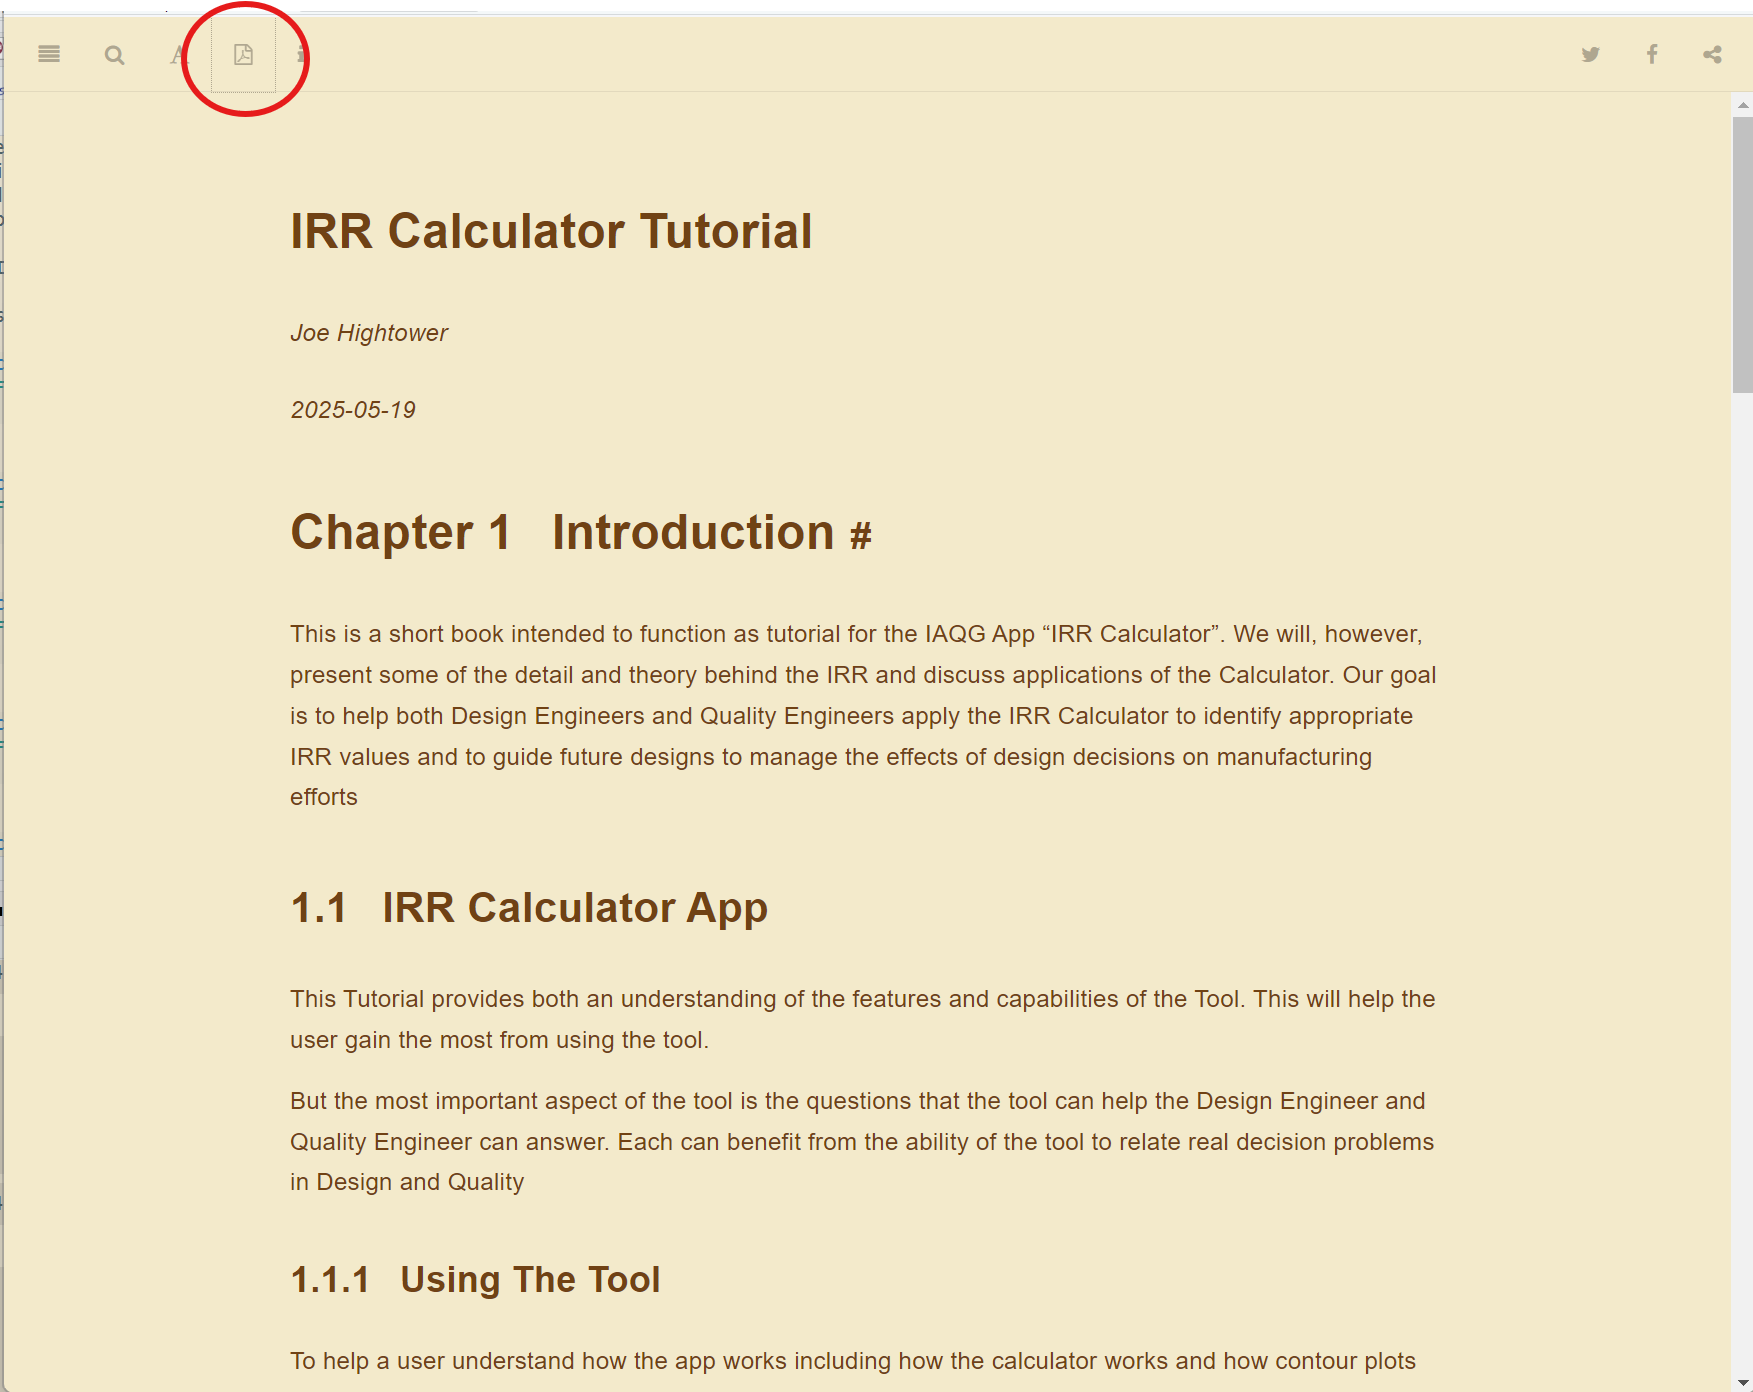
\includegraphics[width=0.5\linewidth]{Download Selection} 

}

\caption{Download Selection}\label{fig:unnamed-chunk-6}
\end{figure}

Finally, in the upper right corner, the user can share pages from the book if desired:

\begin{figure}

{\centering 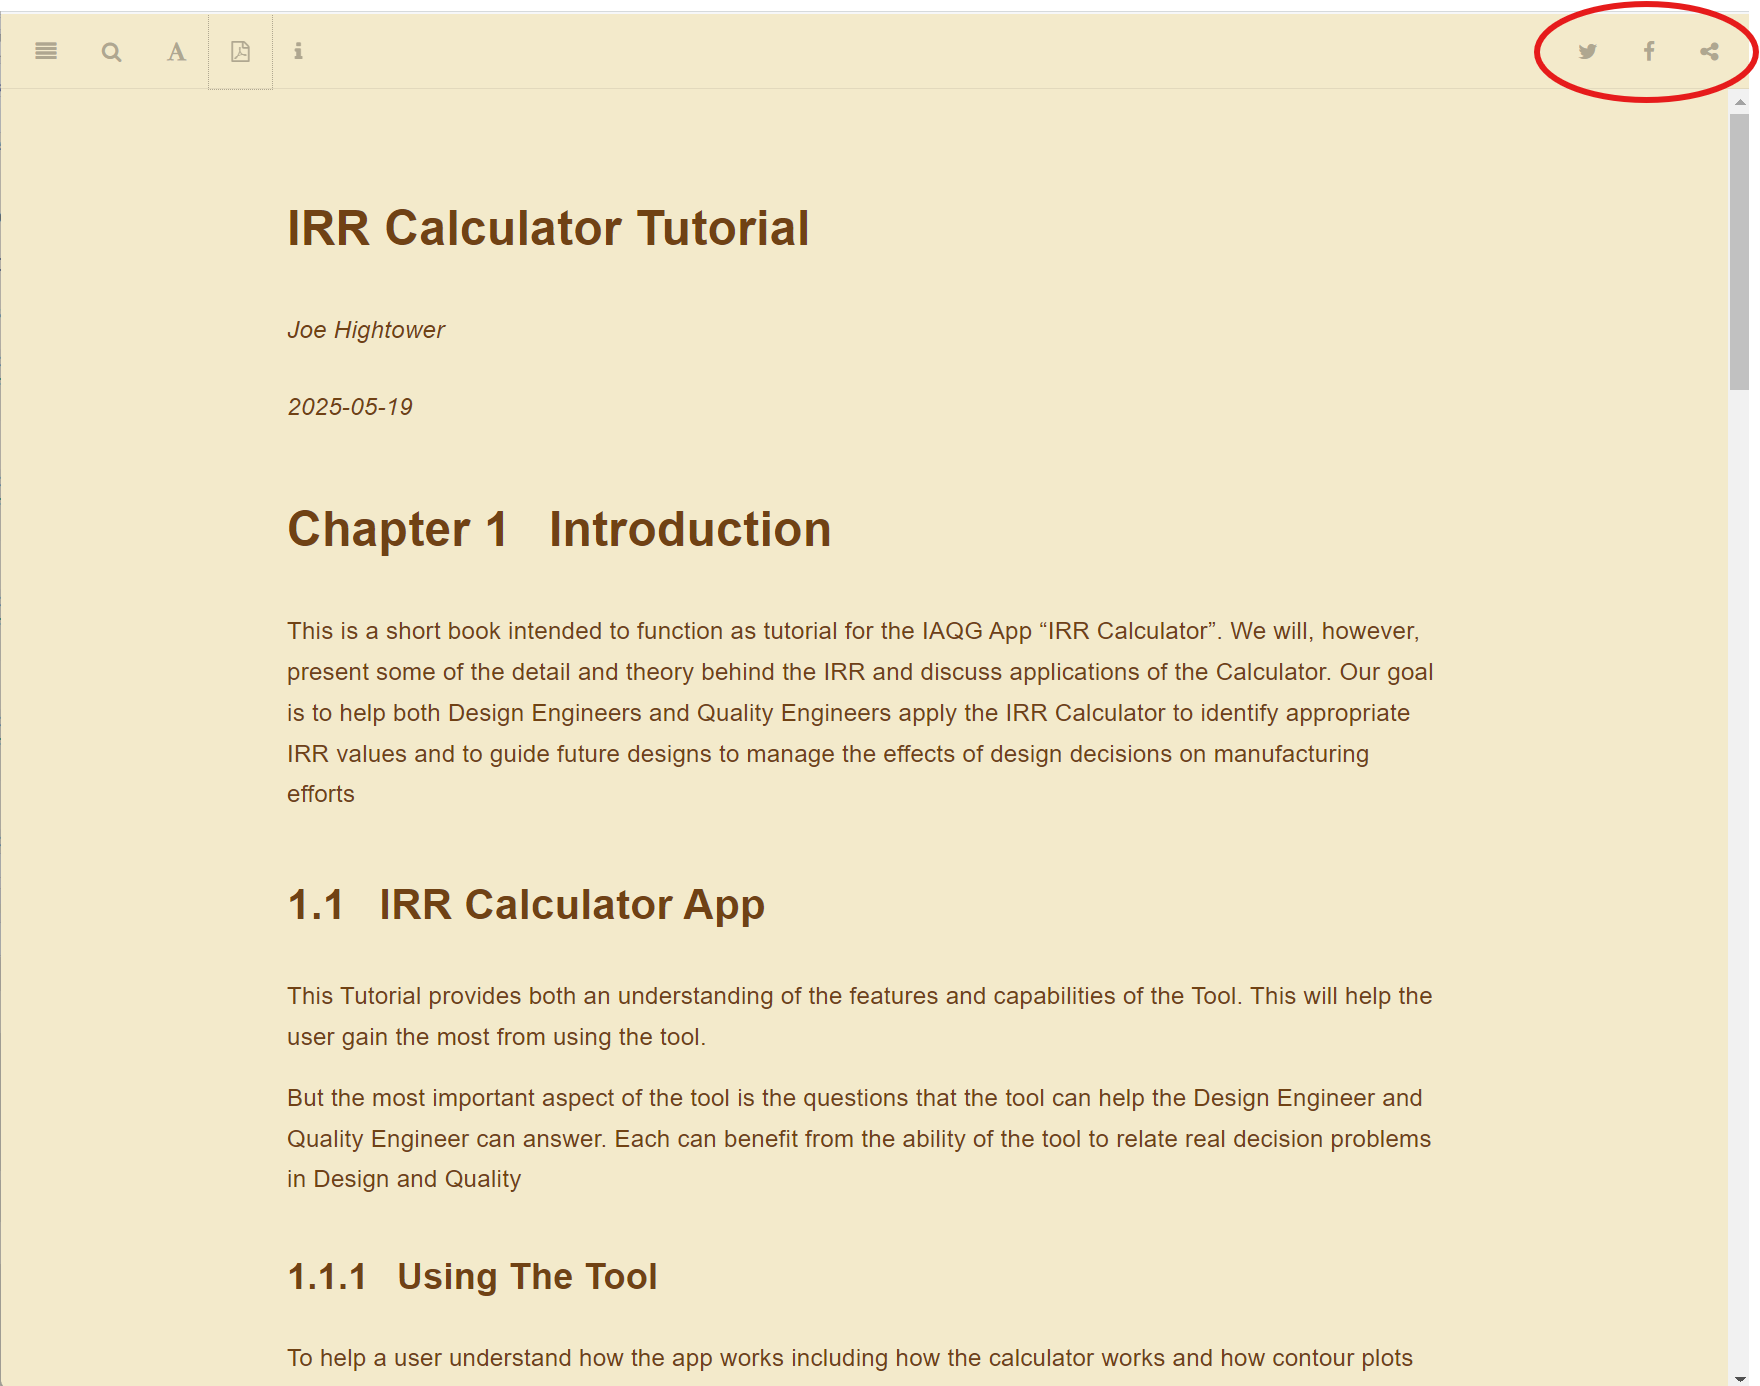
\includegraphics[width=0.5\linewidth]{Sharing} 

}

\caption{Sharing}\label{fig:unnamed-chunk-7}
\end{figure}

Beyond this there is a scrollbar on the right side of the page for scrolling through pages. At the bottom of each page is a set of arrows that allow the user to turn to the next page.

\subsection{Notes on App Layout}\label{notes-on-app-layout}

This tool uses Shiny \citep{R-Shiny}, an interface to provide functionality making data and data activities accessible in an accessible user interface. Underneath the hood is R \citep{R-base}, Which performs the statistical work behind the results the user interacts with.

The Shiny Interface includes the following:

\begin{enumerate}
\def\labelenumi{\arabic{enumi}.}
\tightlist
\item
  A landing page where the App starts out
\end{enumerate}

\begin{figure}

{\centering 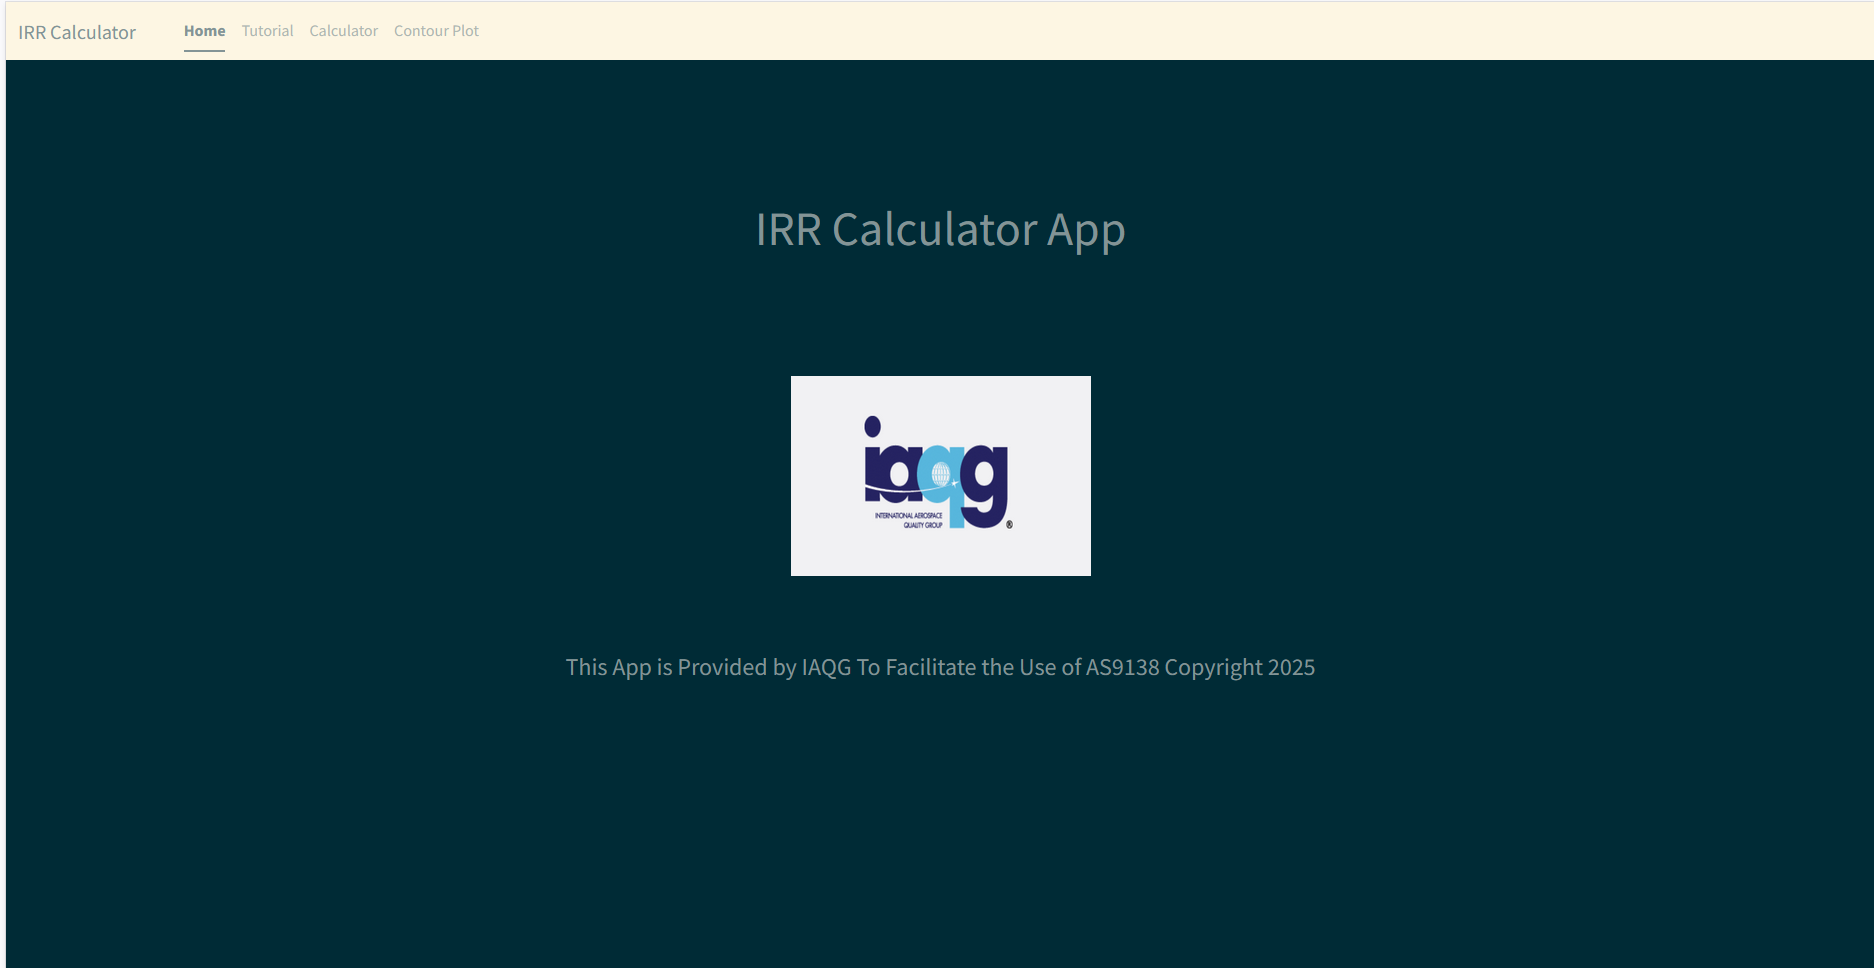
\includegraphics[width=0.5\linewidth]{Landing_Page} 

}

\caption{Sharing}\label{fig:unnamed-chunk-8}
\end{figure}

\begin{enumerate}
\def\labelenumi{\arabic{enumi}.}
\setcounter{enumi}{1}
\tightlist
\item
  From the Landing Page the user can use tabbed sections to access
\end{enumerate}

\begin{enumerate}
\def\labelenumi{\alph{enumi}.}
\tightlist
\item
  This tutorial
\end{enumerate}

\begin{figure}

{\centering 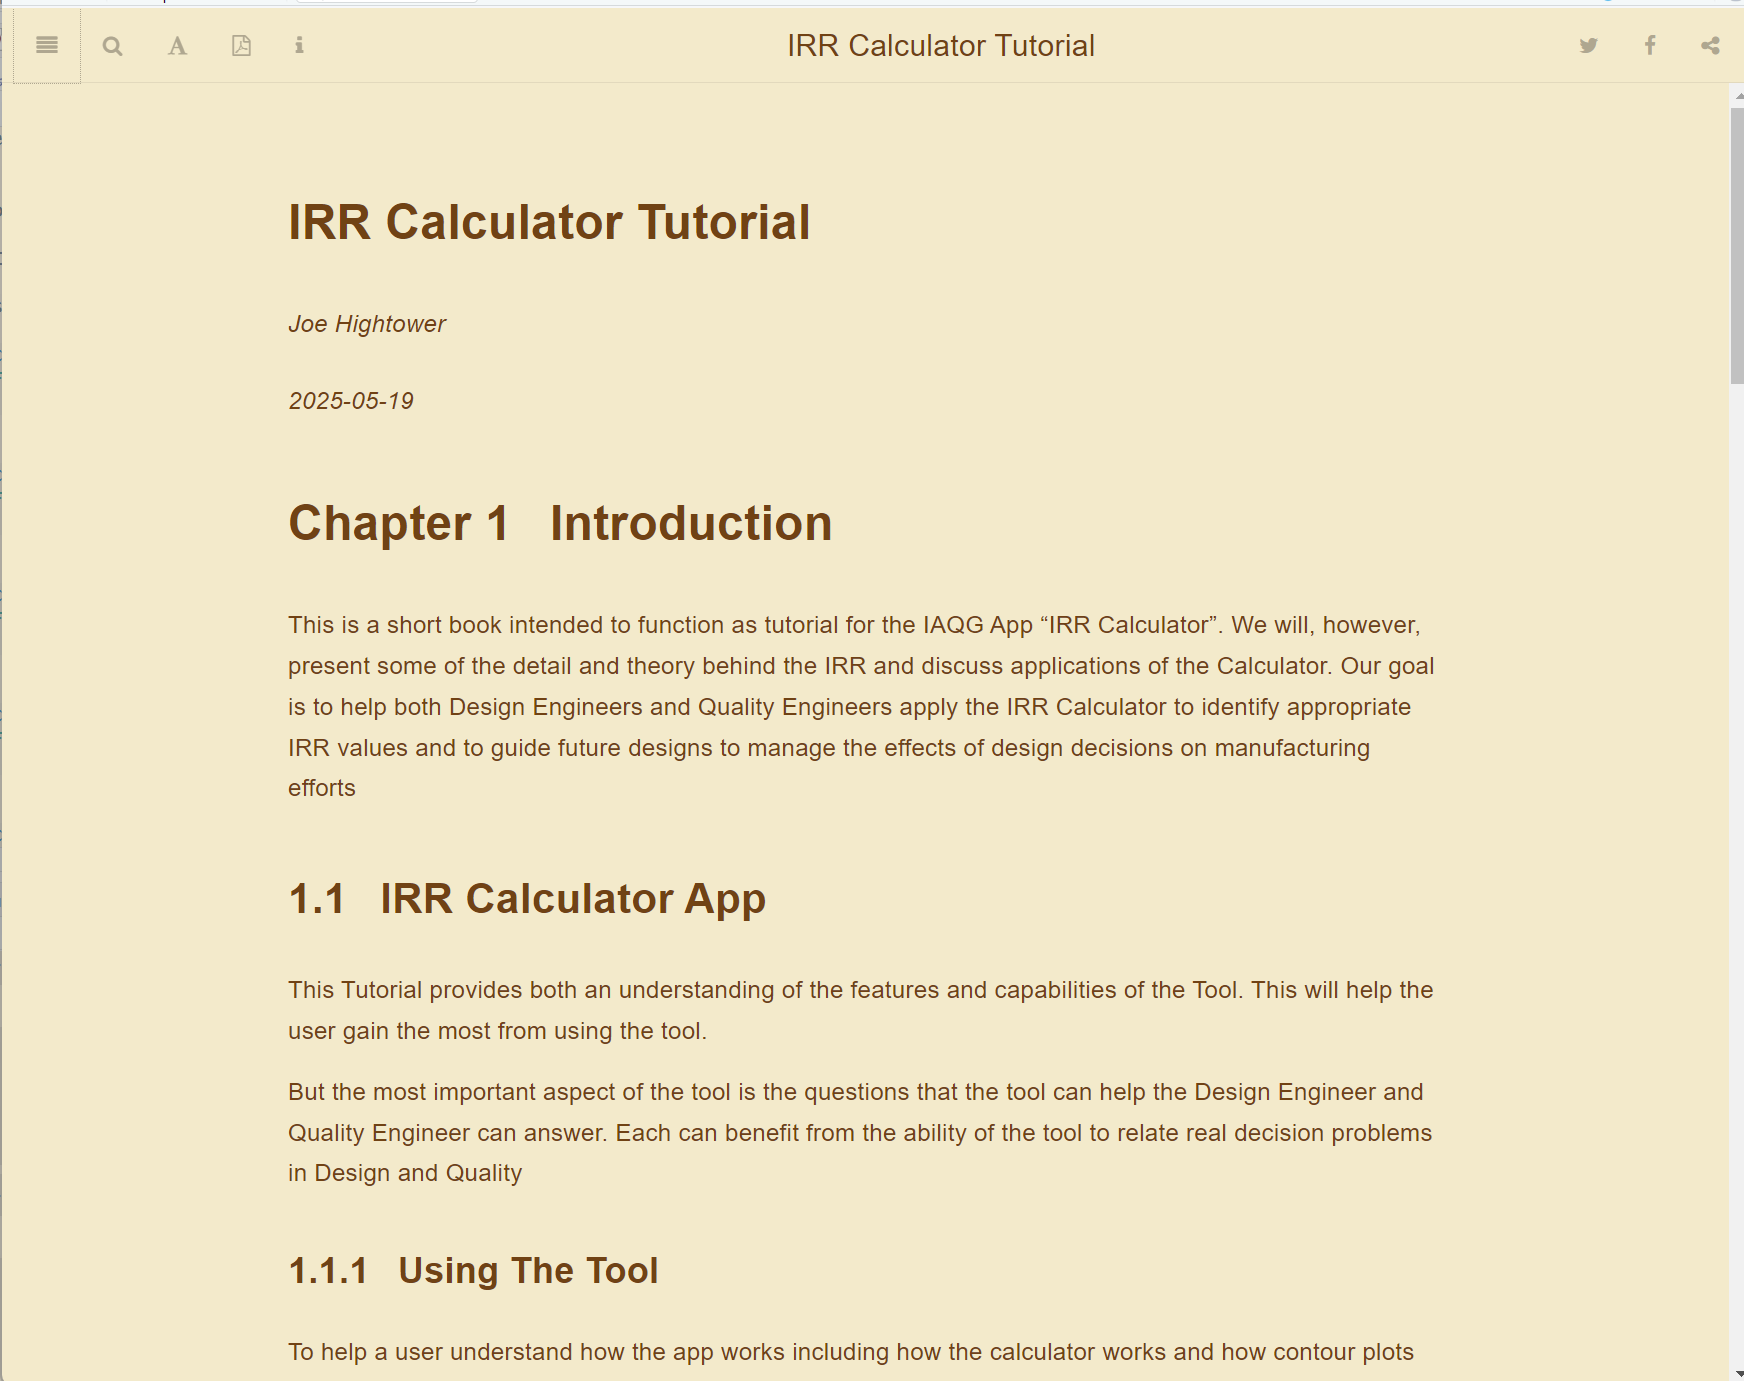
\includegraphics[width=0.5\linewidth]{Main Book Interface} 

}

\caption{Main bookdown Interface}\label{fig:unnamed-chunk-9}
\end{figure}

\begin{enumerate}
\def\labelenumi{\alph{enumi}.}
\setcounter{enumi}{1}
\tightlist
\item
  The IRR Calculator
\end{enumerate}

\begin{figure}

{\centering 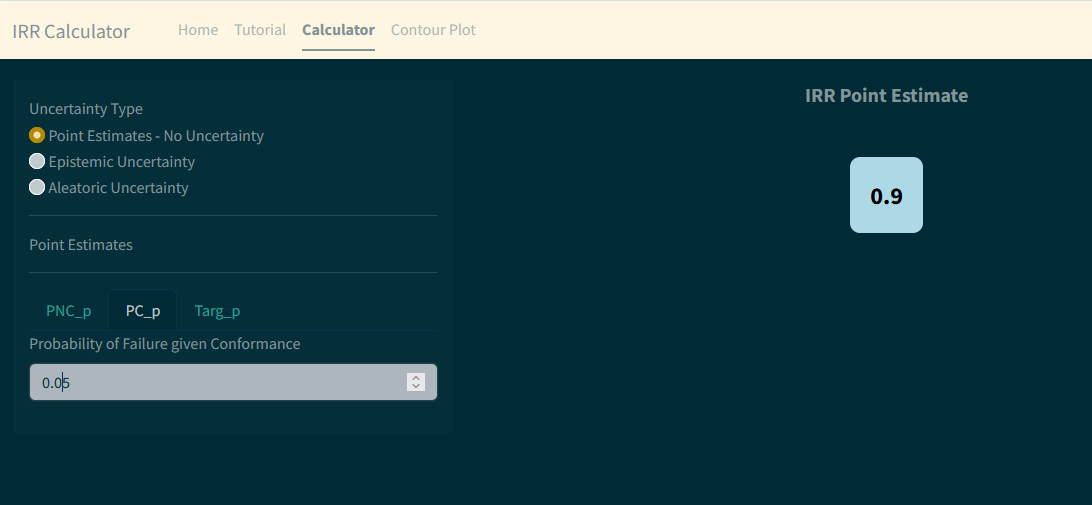
\includegraphics[width=0.5\linewidth]{IRR_Calculator} 

}

\caption{Main bookdown Interface}\label{fig:unnamed-chunk-10}
\end{figure}

\begin{enumerate}
\def\labelenumi{\alph{enumi}.}
\setcounter{enumi}{2}
\tightlist
\item
  The Design Space Explorer
\end{enumerate}

\begin{figure}

{\centering 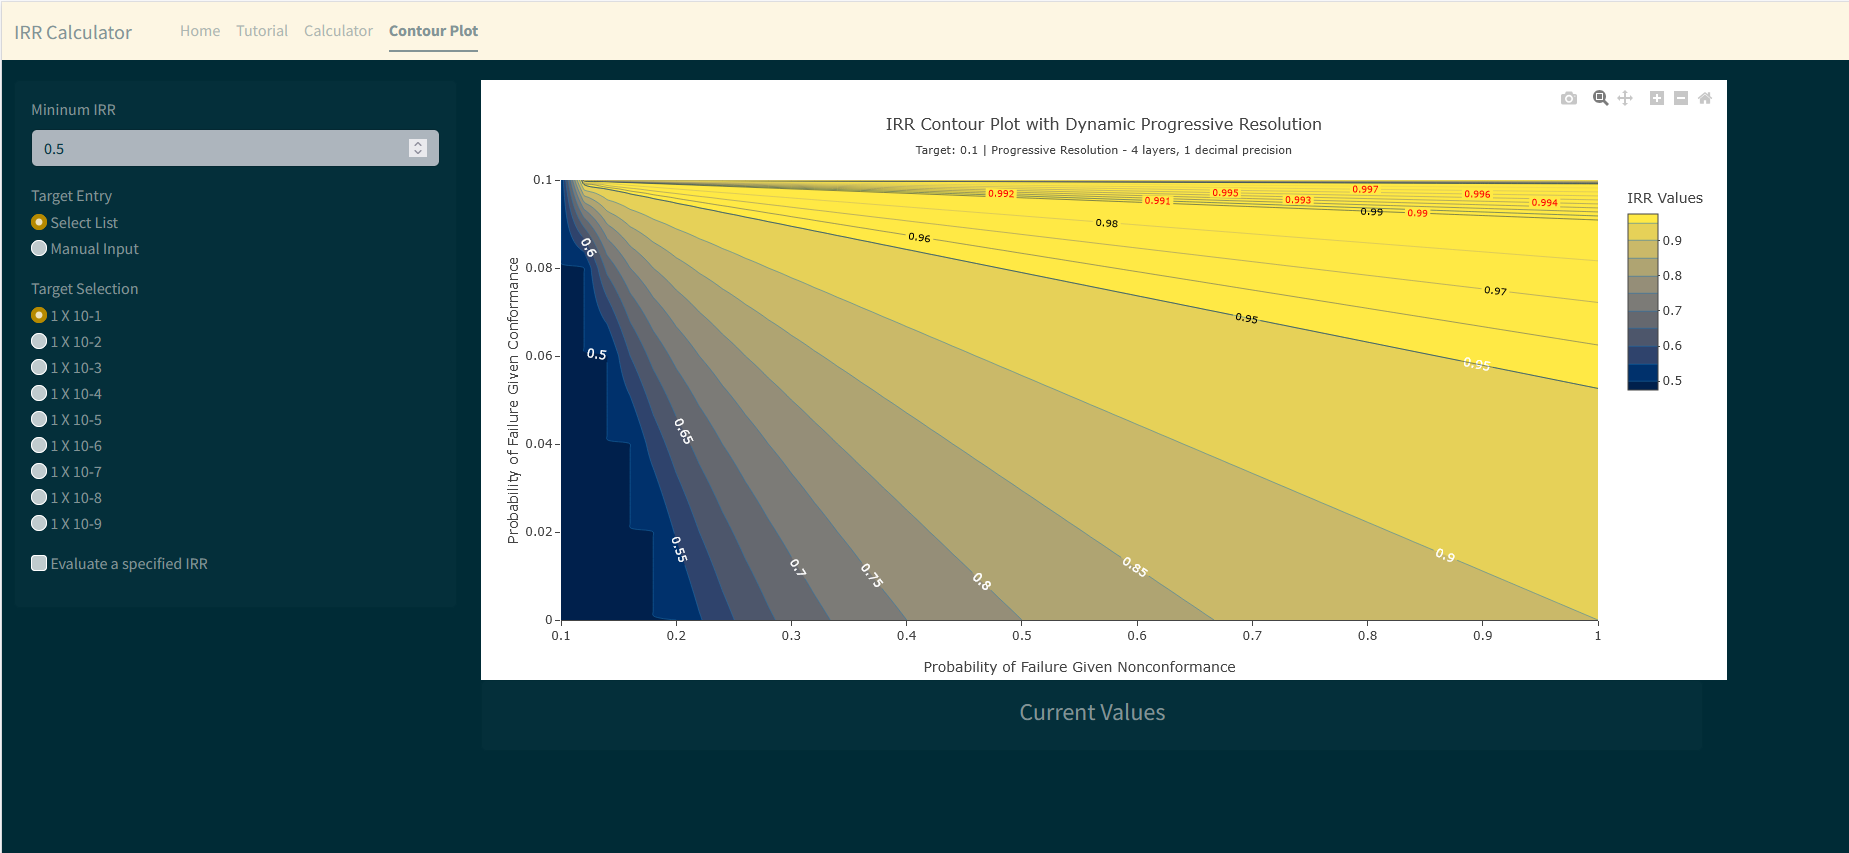
\includegraphics[width=0.5\linewidth]{Design Space Explorer} 

}

\caption{Main bookdown Interface}\label{fig:unnamed-chunk-11}
\end{figure}

\begin{enumerate}
\def\labelenumi{\arabic{enumi}.}
\setcounter{enumi}{2}
\tightlist
\item
  Note that the application is designed to input required parameters on the left side and display results in the main area
\end{enumerate}

\begin{figure}

{\centering 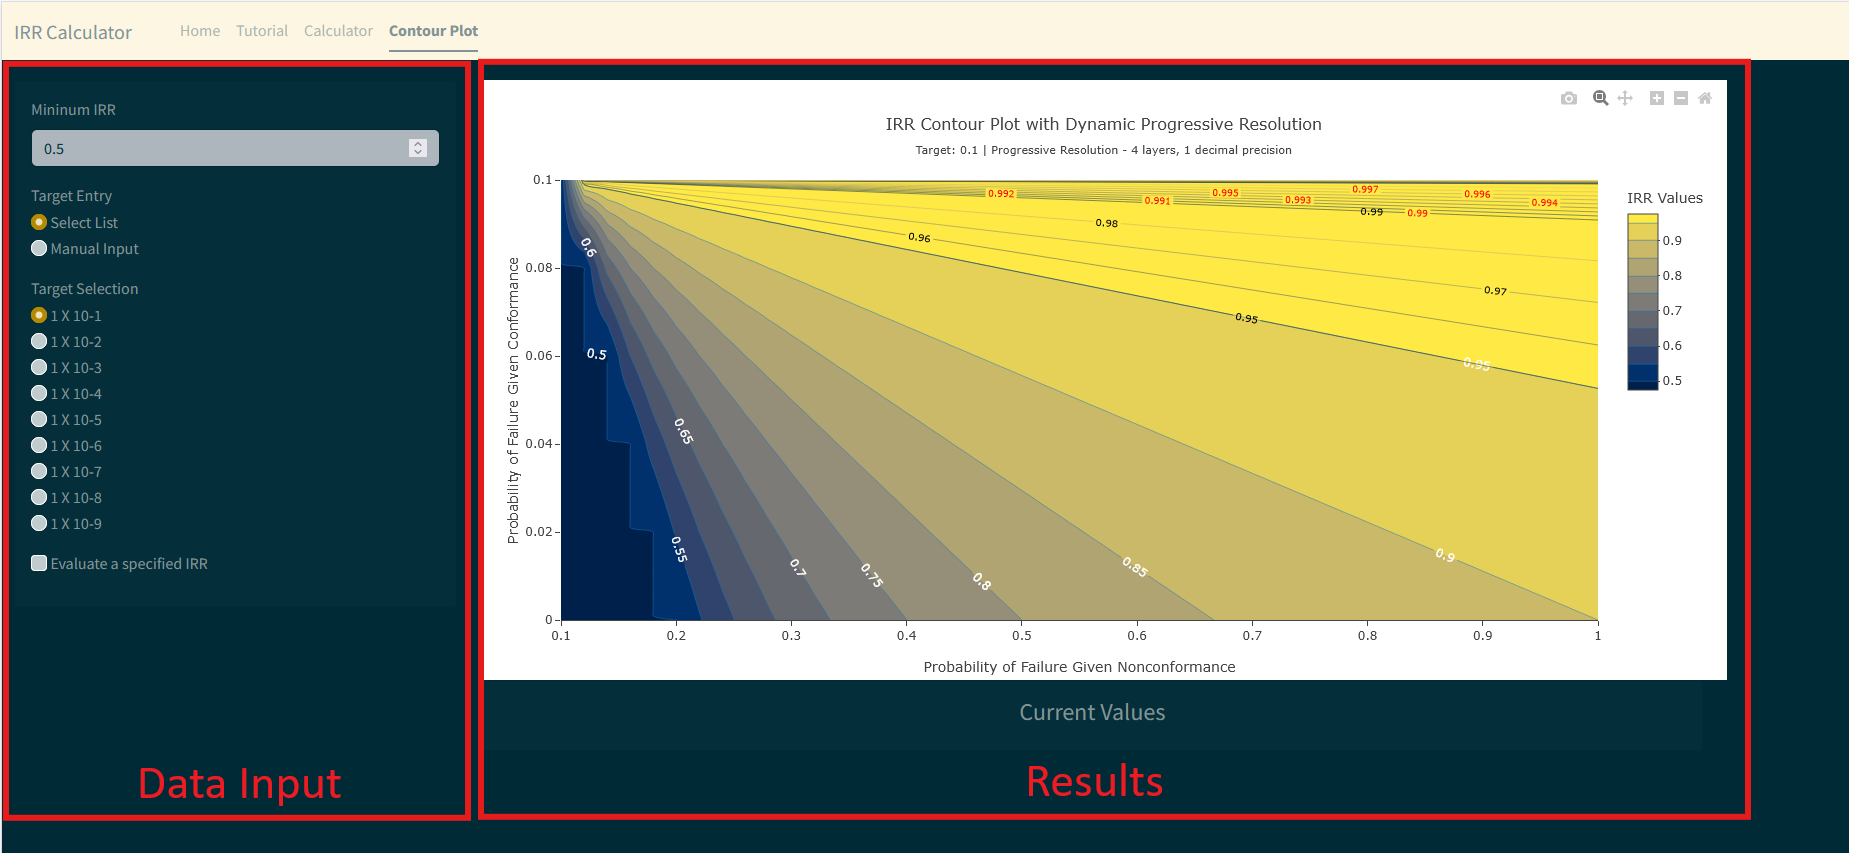
\includegraphics[width=0.5\linewidth]{Page Layout} 

}

\caption{Main bookdown Interface}\label{fig:unnamed-chunk-12}
\end{figure}
\begin{tipbox}
\faLightbulb\ \textbf{Tip:} The Data Input may include additonal tabs separating the three input values where each may require multiple inputs and other settings.
\end{tipbox}

\subsection{Notes on Plots Created in The IRR App}\label{notes-on-plots-created-in-the-irr-app}

This tool uses Plotly R Open Source Graphing Library \citep{plotly}, a graphing library library making publication quality graphs. A key aspect of Plotly graphs is interactivity, through both the cursor and through a toolbar associated with each graph.

Cursor interactivity changes depending on the graph type, but typically will include coordinate information of points where the cursor is located allowing the user to examine the data behind minimum and maximum values, etc.

\begin{figure}

{\centering 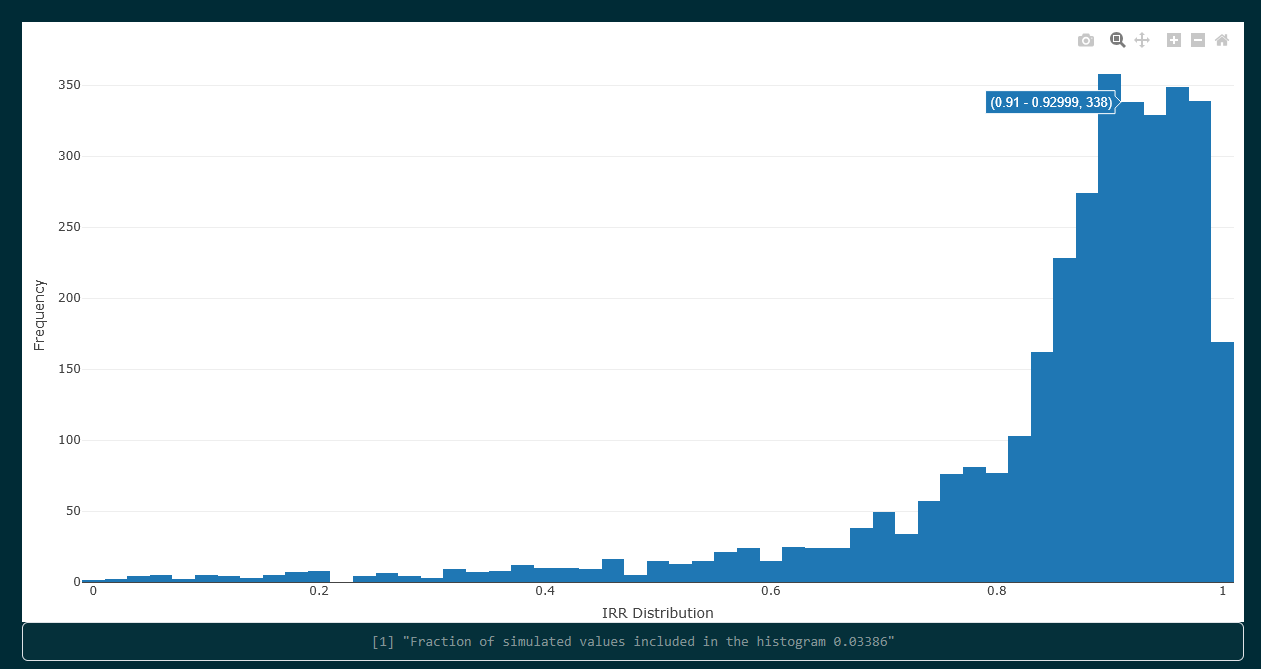
\includegraphics[width=0.5\linewidth]{Cursor Feedback} 

}

\caption{Main bookdown Interface}\label{fig:unnamed-chunk-14}
\end{figure}

The Toolbar is located in the upper right of the plot area. The Toolbar adds several useful tools including the ability to save a copy of the plot as a PNG image file, zoom, pan, and restore the plot to original scale.

\begin{figure}

{\centering 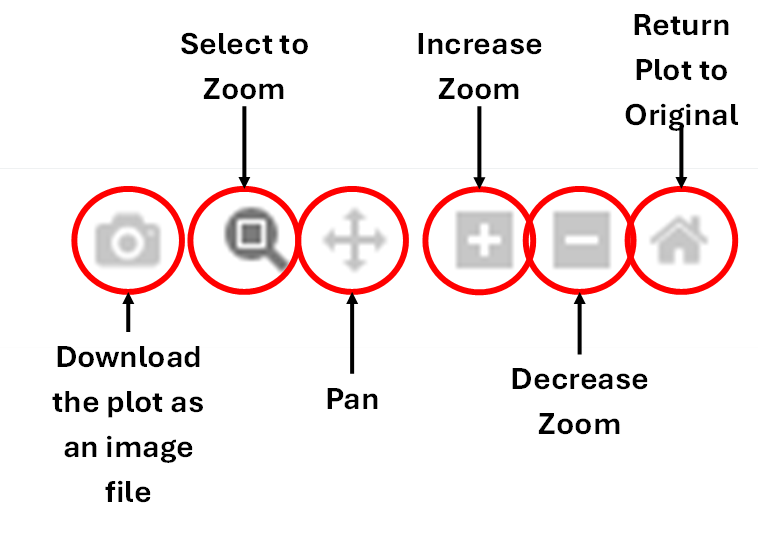
\includegraphics[width=0.5\linewidth]{Plotly Toolbar} 

}

\caption{Main bookdown Interface}\label{fig:unnamed-chunk-15}
\end{figure}

\begin{tipbox}
\faLightbulb\ \textbf{Tip:} The Download Image function captures the image as it appears on the screen.  If the image has been zoomed, panned, or returned to original scale, the captured image will reflect those choices.
\end{tipbox}

\section{IRR Equation}\label{irr-equation}

\begin{infobox}
\faInfoCircle\ \textbf{Info:} This should be a styled into an info box
\end{infobox}

\subsection{Equation for the Total probability of Failure in delivered product}\label{equation-for-the-total-probability-of-failure-in-delivered-product}

We start with the Law of Total Probability, which allows us to partition the Probability of Failure into two parts:

\begin{enumerate}
\def\labelenumi{\arabic{enumi}.}
\item
  The Probability of Failure given Conformance - The probability of failure associated with product that conforms to requirements
\item
  The Probability of Failure given Nonconformance - the probability of failure associated with product that does not conform to requirements
\end{enumerate}

We will label these as

\begin{enumerate}
\def\labelenumi{\arabic{enumi}.}
\tightlist
\item
  \(P_{total}[failure]_{delivered}\) the total probability of failure in the delivered airplane
\item
  \(P[failure|C]_{delivered}\) the probability of failure given conformance in the delivered airplane
\item
  \(P[failure|NC]_{delivered}\) the probability of failure given conformance in the delivered airplane
\end{enumerate}

Note that it is key that all three terms are representing the same scale. For example AC1309-1B measures the probability on a per hour basis. THat would mean that we would also represent \(P[failure|C]_{delivered}\) and \(P[failure|NC]_{delivered}\) on a per hour basis.

\subsubsection{Partitioning the Total Probability of Failure}\label{partitioning-the-total-probability-of-failure}

In Figure 1 we use a Venn diagram to illustrate the partitioning of the probability of failure into two regions.

\begin{figure}

{\centering 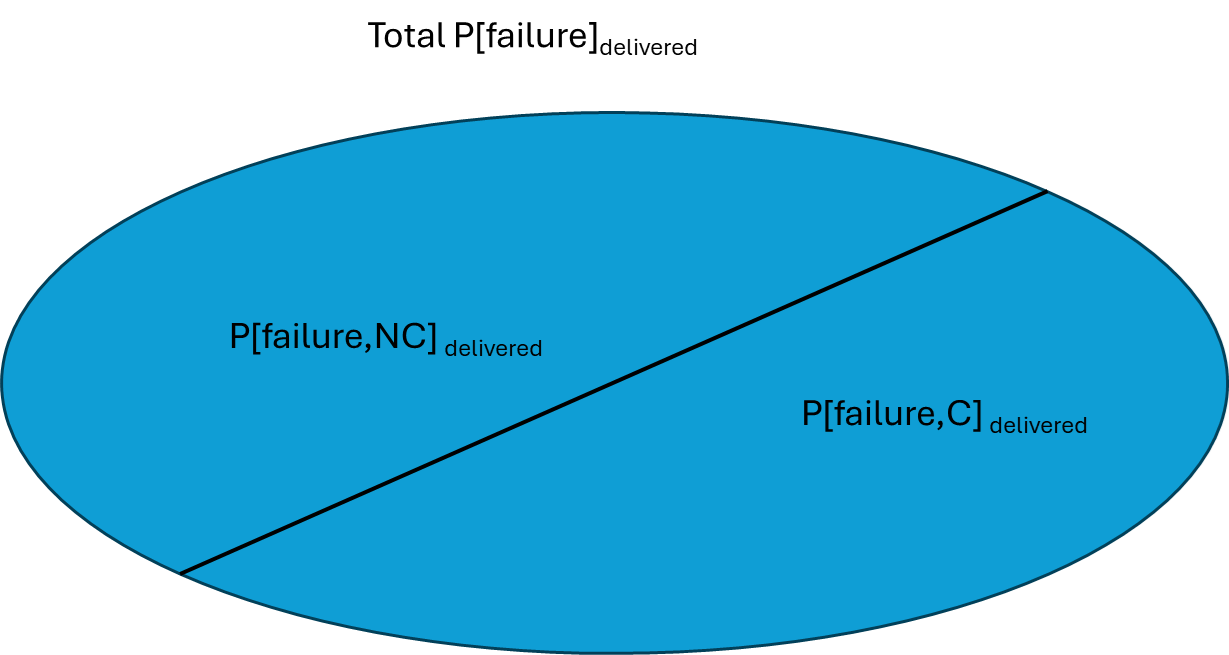
\includegraphics[width=0.5\linewidth]{Figure_1_IRR_Tutorial} 

}

\caption{Venn Diagram Partitioning the space for Total Probability of Failure in delvered product}\label{fig:unnamed-chunk-18}
\end{figure}

The Venn Diagram shows two regions, the first is the joint probability that the prodcut fails and is nonconforming. The second is the joint probability that the product fails and is conforming.

These are represented by

\begin{enumerate}
\def\labelenumi{\arabic{enumi}.}
\tightlist
\item
  \(P[fails,conforming]_{delivered}\)
\item
  \(P[fails,nonconforming]_{delivered}\)
\end{enumerate}

and the total probability of failure is defined as

\[
P_{total}[failure]_{delivered} = P[fails,conforming]_{delivered} + P[fails,nonconforming]_{delivered} \tag{1}
\]

Our next step is to expand the identified joint probabilities using the standard relationship

\[ Joint Probability = Marginal probability * Conditional Probability \]
In this case \(P[fails,conforming]_{delivered}\) expands to

\[ P[fails,conforming] = P[C]_{delivered} * P[failure|C]_{delivered} \]

Then \(P[fails,conforming]_{delivered}\) expands to

\[ P[fails,nonconforming] = P[NC]_{delivered} * P[failure|NC]_{delivered} \]

and now we can make substitutions in Equation X so that we arrive at a useful form in our discusison of the IRR

\[ P_{total}[failure]_{delivered} = P[C]_{delivered} * P[failure|C]_{delivered} + P[NC]_{delivered} * P[failure|NC]_{delivered} \tag{2}\]

\subsection{Linking the equation to a target maximum probability of failure}\label{linking-the-equation-to-a-target-maximum-probability-of-failure}

In the design of product we are most interested in ensuring that \(P_{total}[failure]_{delivered}\) does not exceed some threshold maximum probability of failure. We will call this threshold maximum \(P_{target}[failure]_{delivered}\). Substituting this into our equation results in the following

\[ P_{target}[failure]_{delivered} >= P[failure|C]_{delivered}*P[C]_{delivered} + P[failure|NC]_{delivered}*P[NC]_{delivered} \tag{3}\]
In this form we are required to assess the four terms on the right hand side, making sure that the design decisions that are made do not result in values for these terms where the result will exceed \(P_{target}[failure]_{delivered}\)

\subsection{Rearrangment and the IRR definition}\label{rearrangment-and-the-irr-definition}

A useful relationship for this is to understand that our terms for \ldots{} are statistical complements

\[ P[NC]_{delivered} = 1 -P[C]_{delivered} \]

We are now ready to perform algebraic rearrangement of Equation X, which result in a form that supports our definition of the IRR. When we are finished we arrive at

\[ P[C]_{delivered} >= \frac{P[failure|NC]_{delivered} - P_{target}[failure]_{delivered}}{P[failure|NC]_{delivered} -  P[failure|C]_{delivered}} \tag{4}\]
Finally, we define the IRR as \(P[C]_{delivered}\)

\[ IRR = P[C]_{delivered} \tag{5}\]

\subsection{Notes on PRobabilities}\label{notes-on-probabilities}

Each of the probabilities included are not restricted to point estimates. They may be estimated by functions, which allows for IRR estimates where there is a range of nonconforming or conforming conditions to be evaluated.

\subsubsection{Functions for Conditional Probabilities of Failure}\label{functions-for-conditional-probabilities-of-failure}

\subsubsection{Functions for marginal probabilities resulting from manufacturing}\label{functions-for-marginal-probabilities-resulting-from-manufacturing}

\subsubsection{Aggregating Individual IRR values to create product level IRR values}\label{aggregating-individual-irr-values-to-create-product-level-irr-values}

\subsection{Boundary Conditions}\label{boundary-conditions}

From Equation 4 we can derive three boundary conditions that must be satisfied.

\subsubsection{Axioms of Probability}\label{axioms-of-probability}

First we should understand that the five terms involved in Equation 4 are all probabilities. This requires that we enforce the three axioms of probability:

\begin{enumerate}
\def\labelenumi{\arabic{enumi}.}
\tightlist
\item
  nonnegativity
\item
  normalization
\item
  additivity
\end{enumerate}

If these axioms are not satisified we will not be able to managed the reliability of the product by managing the outgoing quality of the manufacturing system.

\subsubsection{Lower Boundary}\label{lower-boundary}

The lower boundary is set by considering that the First Axiom requires that a probability be nonnegative. Each of these five probabilities cannot be less than 0. We can evaluate the conditions where the IRR or \(P[C]_{delivered}\) is set to 0. OF course, in a simple relationship like this, we would expect 0 when the numerator of the ratio goes to 0:

\[P[failure|NC]_{delivered} - P_{target}[failure]_{delivered} = 0\]
This condition will exist when

\[P[failure|NC]_{delivered} = P_{target}[failure]_{delivered}\]

If for any reason \(P[failure|NC]_{delivered} < P_{target}[failure]_{delivered}\) the axiom of nonnegativity is violated and we will fail to produce a useful IRR value. In other words if this boundary condition is violated we will not be able to managed the reliability of the product by managing the manufacturing system.

\subsubsection{Upper Boundary}\label{upper-boundary}

The upper boundary is set by considering that the Second Axiom requires that a probability be \textgreater= 1. Each of these five probabilities cannot be less than 0. We can evaluate the conditions where the IRR or \(P[C]_{delivered}\) is set to 1. Of course, in a simple relationship like this, we would expect 1 when the numerator of the ratio is equal to the denominator:

\[P[failure|NC]_{delivered} - P_{target}[failure]_{delivered} = P[failure|NC]_{delivered} -  P[failure|NC]_{delivered}\]
This condition will exist when

\[P[failure|C]_{delivered} = P_{target}[failure]_{delivered}\]

If for any reason \(P[failure|C]_{delivered} > P_{target}[failure]_{delivered}\) the axiom of normalization is violated and we will fail to produce a useful IRR value. In other words if this boundary condition is violated we will not be able to manage the reliability of the product by managing the manufacturing system.

\subsubsection{Mathematical Boundary}\label{mathematical-boundary}

Our final boundary condition exists to protect the mathematical integrity of the equation. This is really not derived from the axioms of probability, but from the need to avoid the limitation created when we divide by zero. This occurs when the denominator of the ratio in Equation 4 goes to zero. This in turn goes to the condition where

\[P[failure|NC]_{delivered} - P[failure|NC]_{delivered} = 0\]

with the result that we cannot allow

\[P[failure|NC]_{delivered} = P[failure|NC]_{delivered}\]

If for any reason \(P[failure|NC]_{delivered} = P[failure|NC]_{delivered}\) the divide by 0 restriction is violated and we will fail to produce a useful IRR value. In other words if this boundary condition is violated we will not be able to manage the reliability of the product by managing the manufacturing system.

\subsection{Summary}\label{summary}

\section{Using the Calculator}\label{using-the-calculator}

We will present examples of uses for Design Purpose and Quality Purposes. For each case, it is necessary that the user have three estimates in hand:

\begin{enumerate}
\def\labelenumi{\arabic{enumi}.}
\tightlist
\item
  An Estimate of the probability of failure when the product is delivered nonconforming
\item
  An estimate of the probability of failure when the product is delivered confomring
\item
  An estimate of the maximum probability of failure that the product is designed to allow.
\end{enumerate}

We can use the associated estimates to determine an appropriate IRR value for a given context.

Note: Consider that the resolution of the estimated IRR will depend on the \ldots{}

Note: This manual does not yet cover IRR values for Products. There is an additional level of uncertainty when the IRR is required to address a product with multiple product characteristics. This will be addressed in a future update of the tool.

\subsection{Types of estimates}\label{types-of-estimates}

\subsubsection{Judgement Under Uncertainty}\label{judgement-under-uncertainty}

Evaluating a IRR requires, to some degree, the judgement of the Engineer. We are dealing with a set of decisions regarding the Probability of Failure given conformance and the Probability of failure given nonconformance. These two are necessary for estimating an IRR. In some cases we may want to evaluate how the IRR is influenced by the target maximum probability of failure also.

But in the real world we can only know these values with some degree of uncertainty. That uncertainty propagates into the estimated IRR value. Methods exist for estimating the uncertainty that is propagated in this way.

But in a judgement based decision, we often do not know the uncertainty in our estimates of each the two parameters. This means that we cannot evaluate the propagated uncertainty associated with the IRR.

So how do we reduce the risk associated with this problem? The first and primary approach is to gather the data necessary to estimate the parameter and the uncertainty associated with it. Then we can use simple methods to propagate the uncertainty int the IRR estimate, with the result that we will understand the uncertainty and be able to make decision accordingly.

\subsubsection{First we discuss the relationship to Risk}\label{first-we-discuss-the-relationship-to-risk}

We start by evaluating a table constructed from data presented in AC 25.1309-1b ``System Design and Analysis''. This data applies labels to different probabilities of failure. The labels reflect a perception that as probability of failure decreases by orders of magnitude the expectation of failure conditions decreases. This table is derived from \footnote{AC 25.1309-1b ``System Design And Analysis}

\begin{tabular}{c|c|c}
\hline
Failure.Condition & Upper.Boundary & Lower.Boundary\\
\hline
Likely Failure Condition & $= 1 \times 10^{-1}$ & $> 1 \times 10^{-3}$\\
\hline
Probable Failure Conditions & $= 1 \times 10^{-3}$ & $> 1 \times 10^{-5}$\\
\hline
Remote Failure Conditions & $= 1 \times 10^{-5}$ & $> 1 \times 10^{-7}$\\
\hline
Extremely Remote Failure Conditions & $= 1 \times 10^{-7}$ & $> 1 \times 10^{-9}$\\
\hline
Extremely Improbable Failure Conditions & $= 1 \times 10^{-9}$ & $< 1 \times 10^{-9}$\\
\hline
\end{tabular}

Now to relate this to risk, we would expect that we would set a lower probability failure as a maximum target in order to control the risk to the product and or the customer that results from those failure conditions. ``Extremely Improbable Failure Conditions'' would represent events that are very unlikely to occur, a level we would choose if the risk to the product or the customer for the failure condition is high.

But often, we cannot take the time or the resources to make these estimates. The primary method then is to understand that uncertainty exists and then to manage the decisions we will make accordingly. If we have no knowledge about the uncertainty, we would not want to make decisions where precision is important.

Judgements apart from data are very difficult to make. Simply evaluating an IRR would be extremely difficult. Making the judgement relies on intuition and experience. But it also relies on cognitive biases. These engage beliefs that may or may not be true, they may engage heuristics that causes an engineer to adjust their estimates based on pre-existing beliefs.

Common cognitive biases include:

\begin{enumerate}
\def\labelenumi{\arabic{enumi}.}
\item
  Anchoring biases - The anchoring bias, is the tendency to ``anchor'' on one piece of information when making decisions. If a value is suggested by and expert source, then the decision is anchored to that value even if adjsutments are made. This is often with disregard for differences in context or problem structure.
\item
  Availability Biases - The tendency to overestimate the likelihood of a value based on more recent memory, which can be influenced by how unusual they may be. For instance, a major problem related to the decision addressed in the recent past may cause the decision maker to overemphasize the likelihood of that event recurring.
\item
  Selection Biases - when a sample of information is not statistically representative of the problem
\item
  Confirmation Biases - when the decision maker relies solely on data that confirms pre-existing beliefs and fails to consider all relevant data.
\end{enumerate}

For more discussion and additional cognitive biases see \href{https://en.wikipedia.org/wiki/List_of_cognitive_biases}{List of Cognitive Bias}

Properly calibrating judgements to avoid these biases is essential.

\subsubsection{Point Estimates}\label{point-estimates}

Point estimates exist when a single value for each term is either known or assumed to be known. The Design Engineer will select point values for the probability of failure given conformance and the probability of failure given nonconformance that, in their judgement, represents the design decisions made when the product is certified.

\textbf{Note:} The probability of failure given conformance is reflected in judgement based on product testing required for design certification.

But the usual approach to design certification is only required to test conforming product. Nonconforming product is screened out by definition, meaning that these conditions are not available for testing. The probability of failure given nonconformance truly depend on engineering judgement.

If, however, certification by analysis is used, then simulation results may well exist for both conforming conditions and nonconforming conditions. The Design Engineer may well have access to results that will provide some support for their judgement.

However, no measure of uncertainty is provided.

\textbf{Warning:} This form of estimate does not allow for uncertainty to be assessed in the estimate of the IRR.

This will matter when the IRR is estimated, and the effect of the estimate falls into one of three categories:

\begin{enumerate}
\def\labelenumi{\arabic{enumi}.}
\tightlist
\item
  The estimate is a perfect reflection of the product design decisions and therefore its probability of failure will be satisfied by any inspection system that satisfies the IRR.\\
\item
  The input values are conservative and the required IRR is overestimated. The product is protected, but the the cost of inspection will be increased above optimum.
\item
  The input values will be liberal and the required IRR will be underestimated. The product is not protected and the probability of failure will not be achieved, driving cost to the customer.
\end{enumerate}

\paragraph{Epistemic estimates}\label{epistemic-estimates}

If the probability of failure is bounded by a design engineer's experience or beliefs, we have what is called an epistemic estimate of the values. We do not know the actual values, but we are able to establish an expected upper and lower limit for the estimate. We also do not know the distribution of possible values that could exist between these values. IN this context it is best to not supply more than the boundary conditions, making no assumptions about possible distributions. The IRR estimates then establish a bounded region within which we belief that the true IRR will lie.

\paragraph{Aleatoric Estimates}\label{aleatoric-estimates}

These estimates are based on data, with enough data accumulated to estimate the distribution of values within which true value is likely to fall. This form of estimate is called aleatoric.

We will use the distributions for each of the three input parameters to generate a sampling distribution for the IRR. From this distribution we can select a parameter that meets selected criteria. For instance we can select the most conservative IRR where the value is greater than or equal to 90\%, 95\% or most conservatively 99\% of the distribution of IRR values.

\subsection{Using the Calculator for Design Purposes}\label{using-the-calculator-for-design-purposes}

A Design Engineer will use this tool to answer two questions:

\begin{enumerate}
\def\labelenumi{\arabic{enumi}.}
\tightlist
\item
  Given a known value for PNC and PC, for a specified target value, what IRR will we achieve
\item
  For a specified IRR and Target, what values of PNC and PC are required - the tool will not work for this task - the contour plots are more useful.
\end{enumerate}

The Design Engineer may well have an already existing design. This situation will arise when a request is made for an IRR where data is not available. The Design Engineer has three choices for identifying an acceptable IRR:

\begin{enumerate}
\def\labelenumi{\arabic{enumi}.}
\tightlist
\item
  use a judgement based estimate of the three input parameters
\item
  use epistemic boundaries to account for the uncertainty in the engineers knowledge
\item
  Gather data and estimate the three parameters.
\end{enumerate}

These represent decreasing uncertainty, both in terms of magnitude and in terms of knowledge. With point estimates no uncertainty is represented or its effect on IRR estimates is se the uncertainty associated with these estimates to propagate uncertainty into the estimated IRR. Epistemic uncertainties still represent judgement, but uncertainty is introduced into the estimate of the IRR by providing boundaries within which the we demonstrate a range of possible values. Finally, where the input values are estimated from data, we have a full accounting of the uncertainty in the estimates and can use simulation to estimate the resulting uncertainty in our IRR estimate.

With this in mind, we recommend that point estimates be used only when the target maximum probability of failure coincides with the Likely Failure Condition Category. We would recommend that Epistemic uncertainties be applied only to Likely Failure Conditions or to Probable Failure Conditions. Neither of these two approaches should be applied to conditions where the target maximum is is 1 x e-5 of greater.

Then we recommend that data driven estimates be required for all values \textless= 1 x e-5.

It is beyond the scope of this document to present the data that justifies these recommendations, we plan to add this to SCMH documentation in the future.

\subsubsection{Point Estimates}\label{point-estimates-1}

Point Estimates are only useful for low risk conditions. We would recommend that this method of evaluating a product and its relationship to the IRR only for Likely Failure Conditions.

The Design Engineer identifies values for the probability of failure given conformance, and the probability of failure given nonconformance.

\subsubsection{Epistemic Boundaries}\label{epistemic-boundaries}

Epistemic boundaries are constructed by estimating the minimum and maximum values expected by the Engineer for the probability of failure given conformance and the probability of failure given nonconformance. IF the target maximum probability of failure is also uncertain, then upper and lower boundaries can be added for this also.

When combined, these should produce a total of four (eight) IRR estimates. These four (eight) estimates represent the range of IRR values that the engineer expects to bound the IRR. The final step in the process is to select the IRR that provides the maximum protection to the product, which would be the maximim IRR represented in the range.

\subsubsection{Aleatoric Estimates}\label{aleatoric-estimates-1}

\subsection{Using the Calculator for Quality Purposes}\label{using-the-calculator-for-quality-purposes}

Note that it is possible to suggest a starting point with Design Engineers based on Appendix A in AS9138. This tool then can be used to assess whether that IRR is acceptable given the Design Engineers input for our three parameters.

It is also possible to start discussion by estimating the AOQ for an existing inspection method then discussing the results with the Design Engineer. In many cases the linkage between the two may not be clear and enough information may not be available to support a judgment

\section{Comparing Design Space}\label{comparing-design-space}

\subsection{Comparing Design Space For Design Purposes}\label{comparing-design-space-for-design-purposes}

Now is the TIme for all good men to come to the aid of their fellows

\subsection{Comparing Design Space For Quality Purposes}\label{comparing-design-space-for-quality-purposes}

Now is the TIme for all good men to come to the aid of their fellows

\section{Additional Notes}\label{additional-notes}

these will be added

\subsection{xyz}\label{xyz}

Now is the TIme for all good men to come to the aid of their fellows

\subsubsection{Examples of warnings and notes}\label{examples-of-warnings-and-notes}

Point estimates do not account for the uncertainty in the information the decision maker has available. Each input term has either epistemic or aleatoric uncertainty associated, which in turn creates a range of possible \textit{IRR} Values

\begin{infobox}
\faInfoCircle\ \textbf{Info:} This is important information to remember.
\end{infobox}

\begin{warningbox}
\faExclamationTriangle\ \textbf{Warning:} Be careful when running this code.
\end{warningbox}

\begin{tipbox}
\faLightbulb\ \textbf{Tip:} Here's a helpful tip for better results.
\end{tipbox}

\begin{errorbox}
\faTimesCircle\ \textbf{Error:} This shows what happens when something goes wrong.
\end{errorbox}

\section{Glossary}\label{glossary}

\subsection{Epistemic Unceertainty}\label{epistemic-unceertainty}

Epistemic uncertainty is also known as systematic uncertainty, and is due to things one could in principle know but does not in practice. This may be because a measurement is not accurate, because the model neglects certain effects, or because particular data have been deliberately hidden.

taken from Wikipedia article ``Uncertianty Quantification'' \url{https://en.wikipedia.org/wiki/Uncertainty_quantification}

\subsection{Maximum Allowable Probability of Failure}\label{maximum-allowable-probability-of-failure}

A target that limits the probability of failure the product can experience during its assigned mission. This can range from minimal impact (\textgreater10-3), probable (\textless= 10-3, \textgreater{} 10-5), remote (\textless= 10-5, \textgreater{} 10-7), extremely remote (\textless= 10-7, \textgreater10-9), extremely improbable (\textless= 10-9).

taken from AC-1309-1B

\section{References}\label{references}

\addcontentsline{toc}{section}{References}

\nocite{*}\renewcommand{\bibname}{References}\vspace{-2em}

  \bibliography{book.bib,packages.bib}

\end{document}
